\begin{appendices}
\addtocontents{toc}{\protect\renewcommand{\protect\cftchappresnum}{Appendix }}

\newpage
\setcounter{opagenum}{\thepage}
\chapter[Publication III]{Publication III: Modulating the porosity of carbons for improved adsorption of hydrogen, carbon dioxide, and methane: a review}\label{ap:review}

\textbf{Contribution of the author}: The author designed and performed the literature review and wrote the manuscript.

\clearpage
%\BackupCounterGroup[backup-id=pub1]{pagebackup}
\newpage

\setlength{\originalVOffset}{\voffset}   
\setlength{\originalHOffset}{\hoffset}

\setlength{\voffset}{0cm}
\setlength{\hoffset}{0cm}
% too big for overleaf, try compilation later.
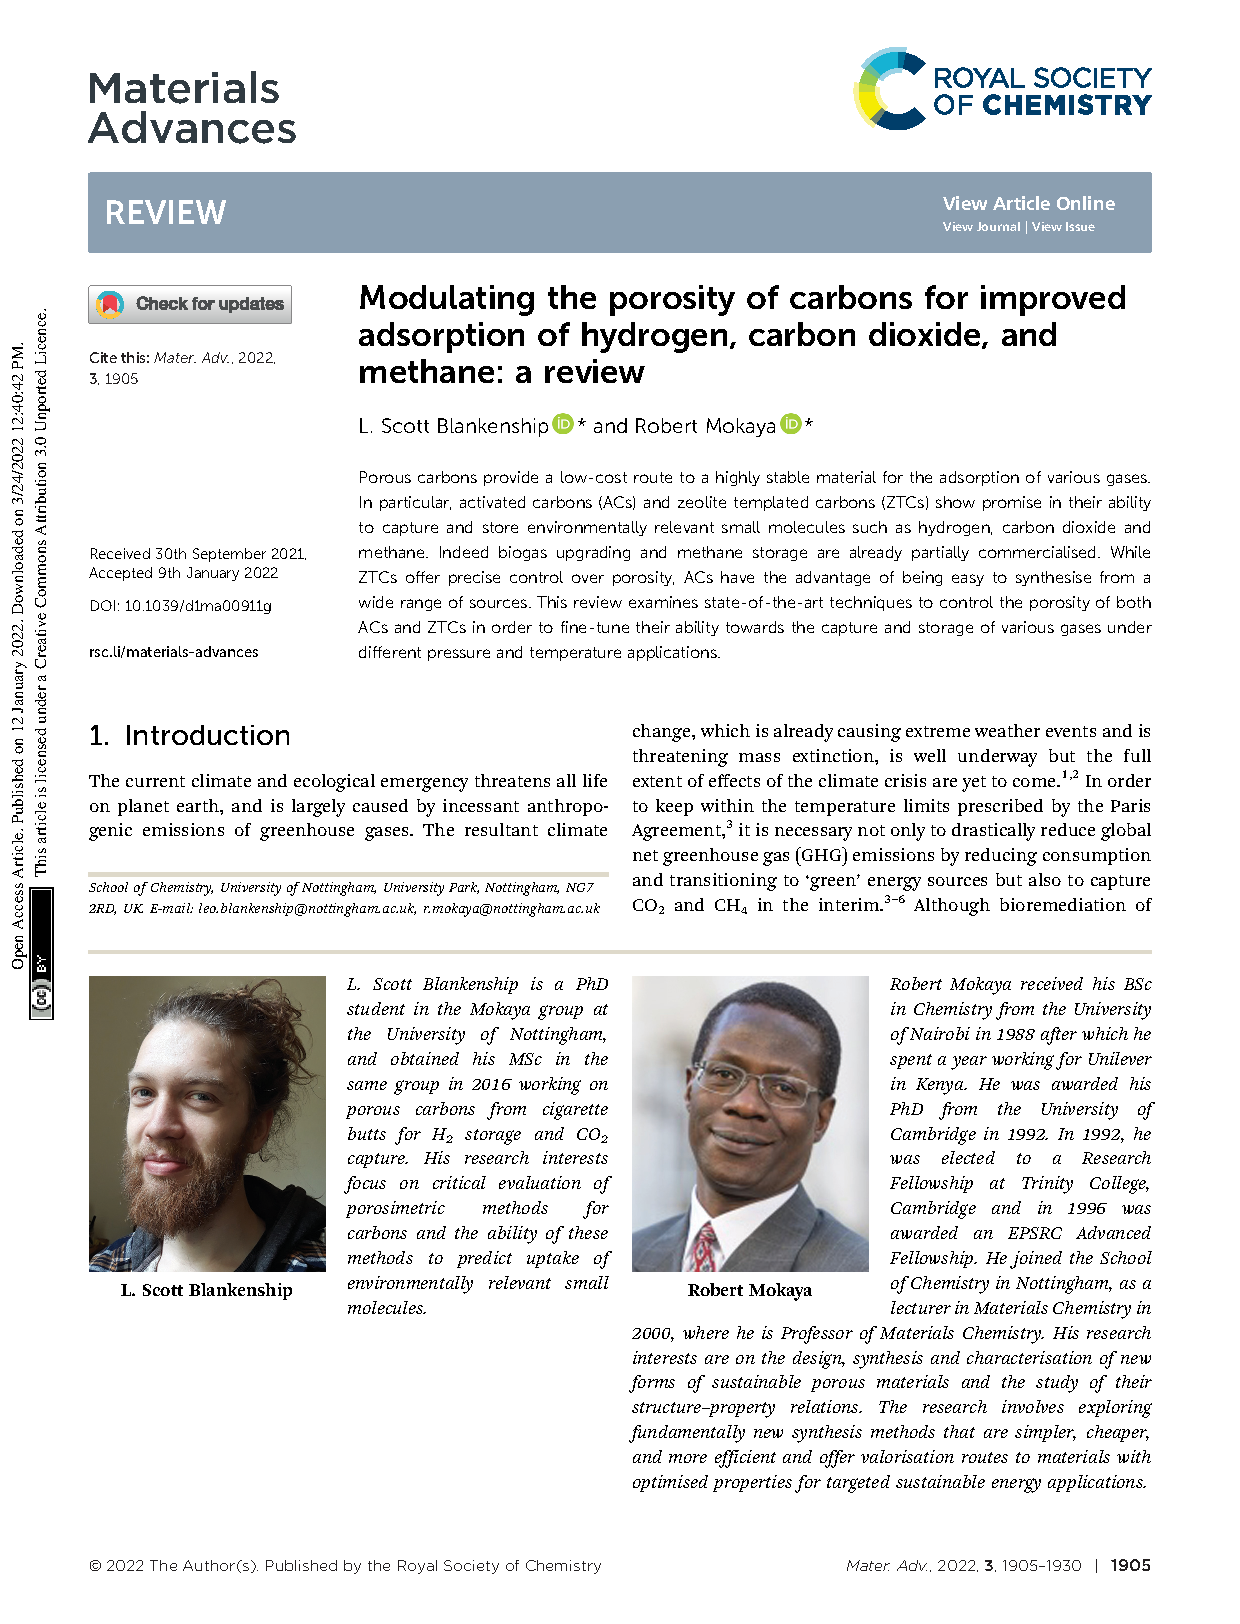
\includepdf[
    pagecommand={
    \setcounter{page}{\theopagenum}
    \thispagestyle{empty}
    },
    pages=-]{1-introduction/publication_01.pdf}
\setlength{\voffset}{\originalVOffset}
\setlength{\hoffset}{\originalHOffset}

\clearpage
%\RestoreBackupCounterGroup[backup-id=pub1]{pagebackup}

\chapter{Compositional Analyses}
\newpage
\begin{figure}[h]
    \centering
    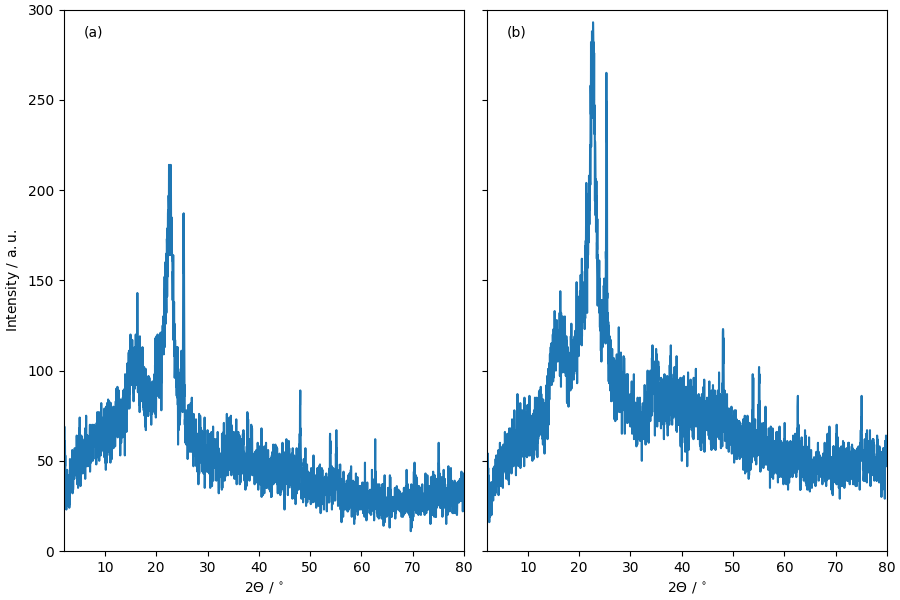
\includegraphics[width=\columnwidth, keepaspectratio]{4-cbs/figs/xrd_hydrochar.png}
    \caption{P-XRD spectra for samples hC-hydrochar (a) and hD-hydrochar (b).}
    \label{fig:xrd_hydrochar}
\end{figure}

\begin{figure}[h]
    \centering
    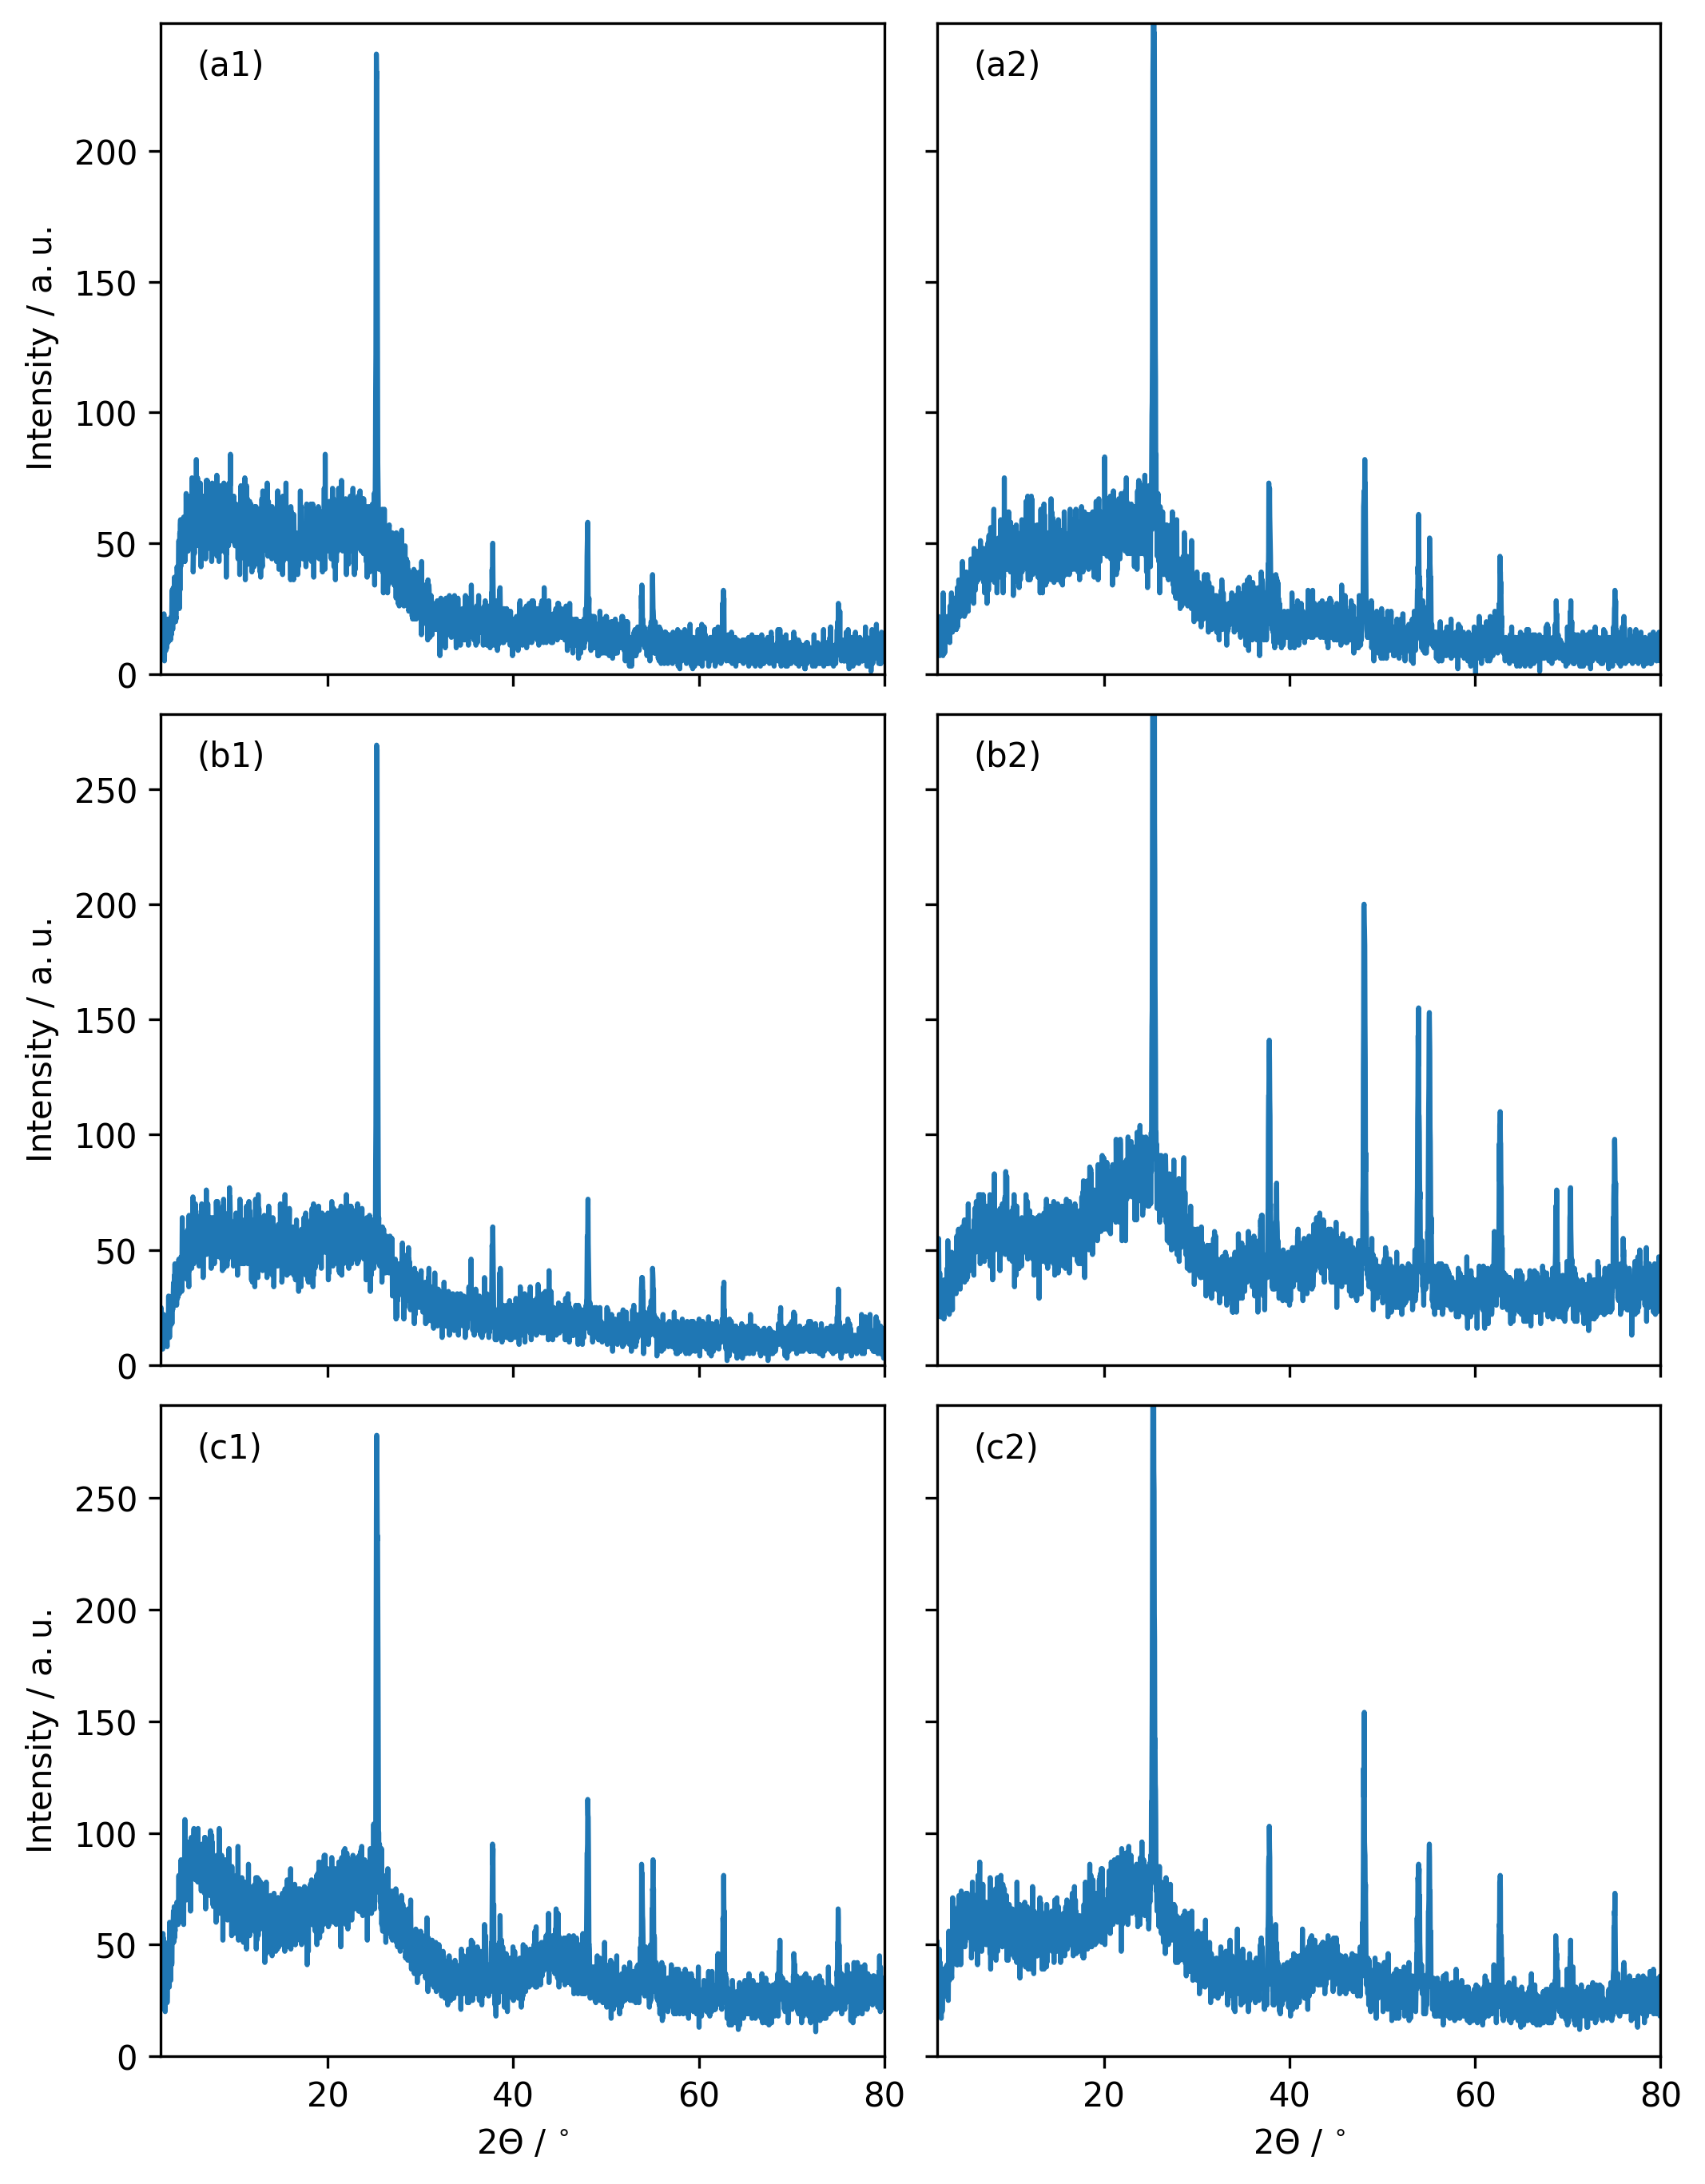
\includegraphics[width=\columnwidth, keepaspectratio]{4-cbs/figs/xrd_hC-0TTT.png}
    \caption{P-XRD spectra for samples hC-0600 (a1), hC-0600$'$ (a2), hC-0700 (b1), hC-0700$'$ (b2), hC-0800 (c1), hC-0800$'$ (c2).}
    \label{fig:xrd_hC-0TTT}
\end{figure}

\begin{figure}[h]
    \centering
    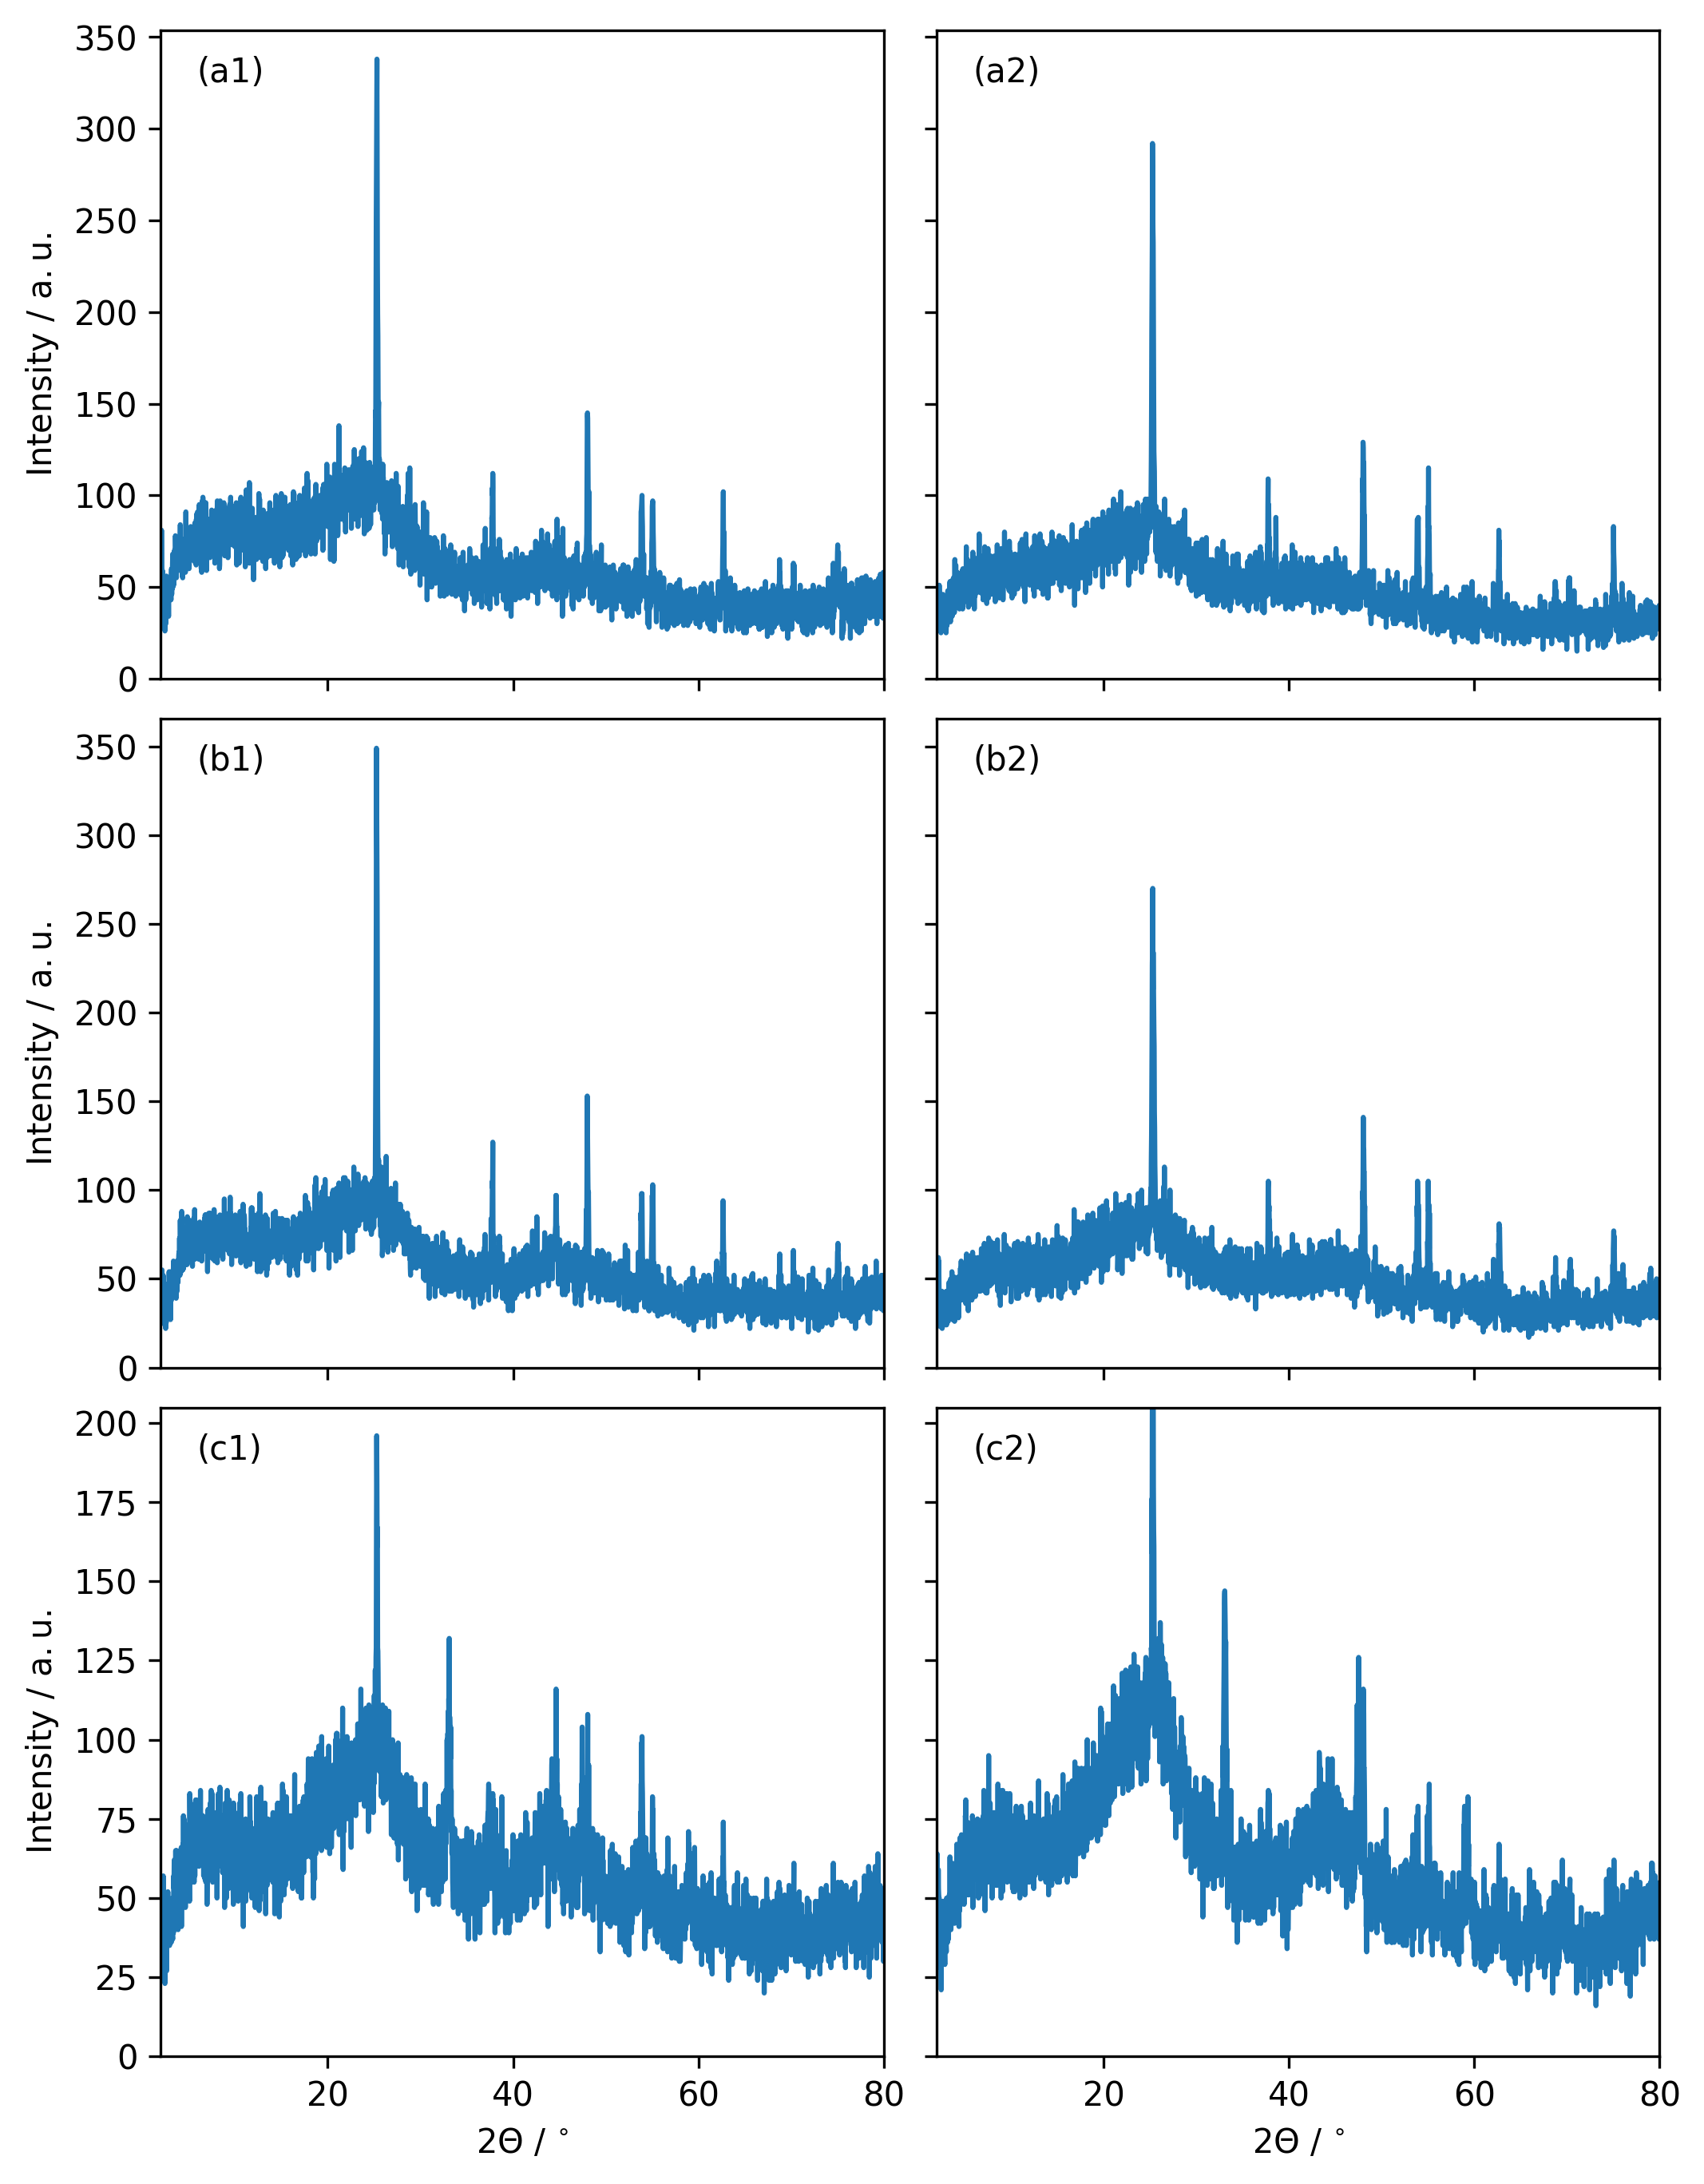
\includegraphics[width=\columnwidth, keepaspectratio]{4-cbs/figs/xrd_hD-0TTT.png}
    \caption{P-XRD spectra for samples hD-0600 (a1), hD-0600$'$ (a2), hD-0700 (b1), hD-0700$'$ (b2), hD-0800 (c1), hD-0800$'$ (c2).}
    \label{fig:xrd_hD-0TTT}
\end{figure}

\begin{figure}[h]
    \centering
    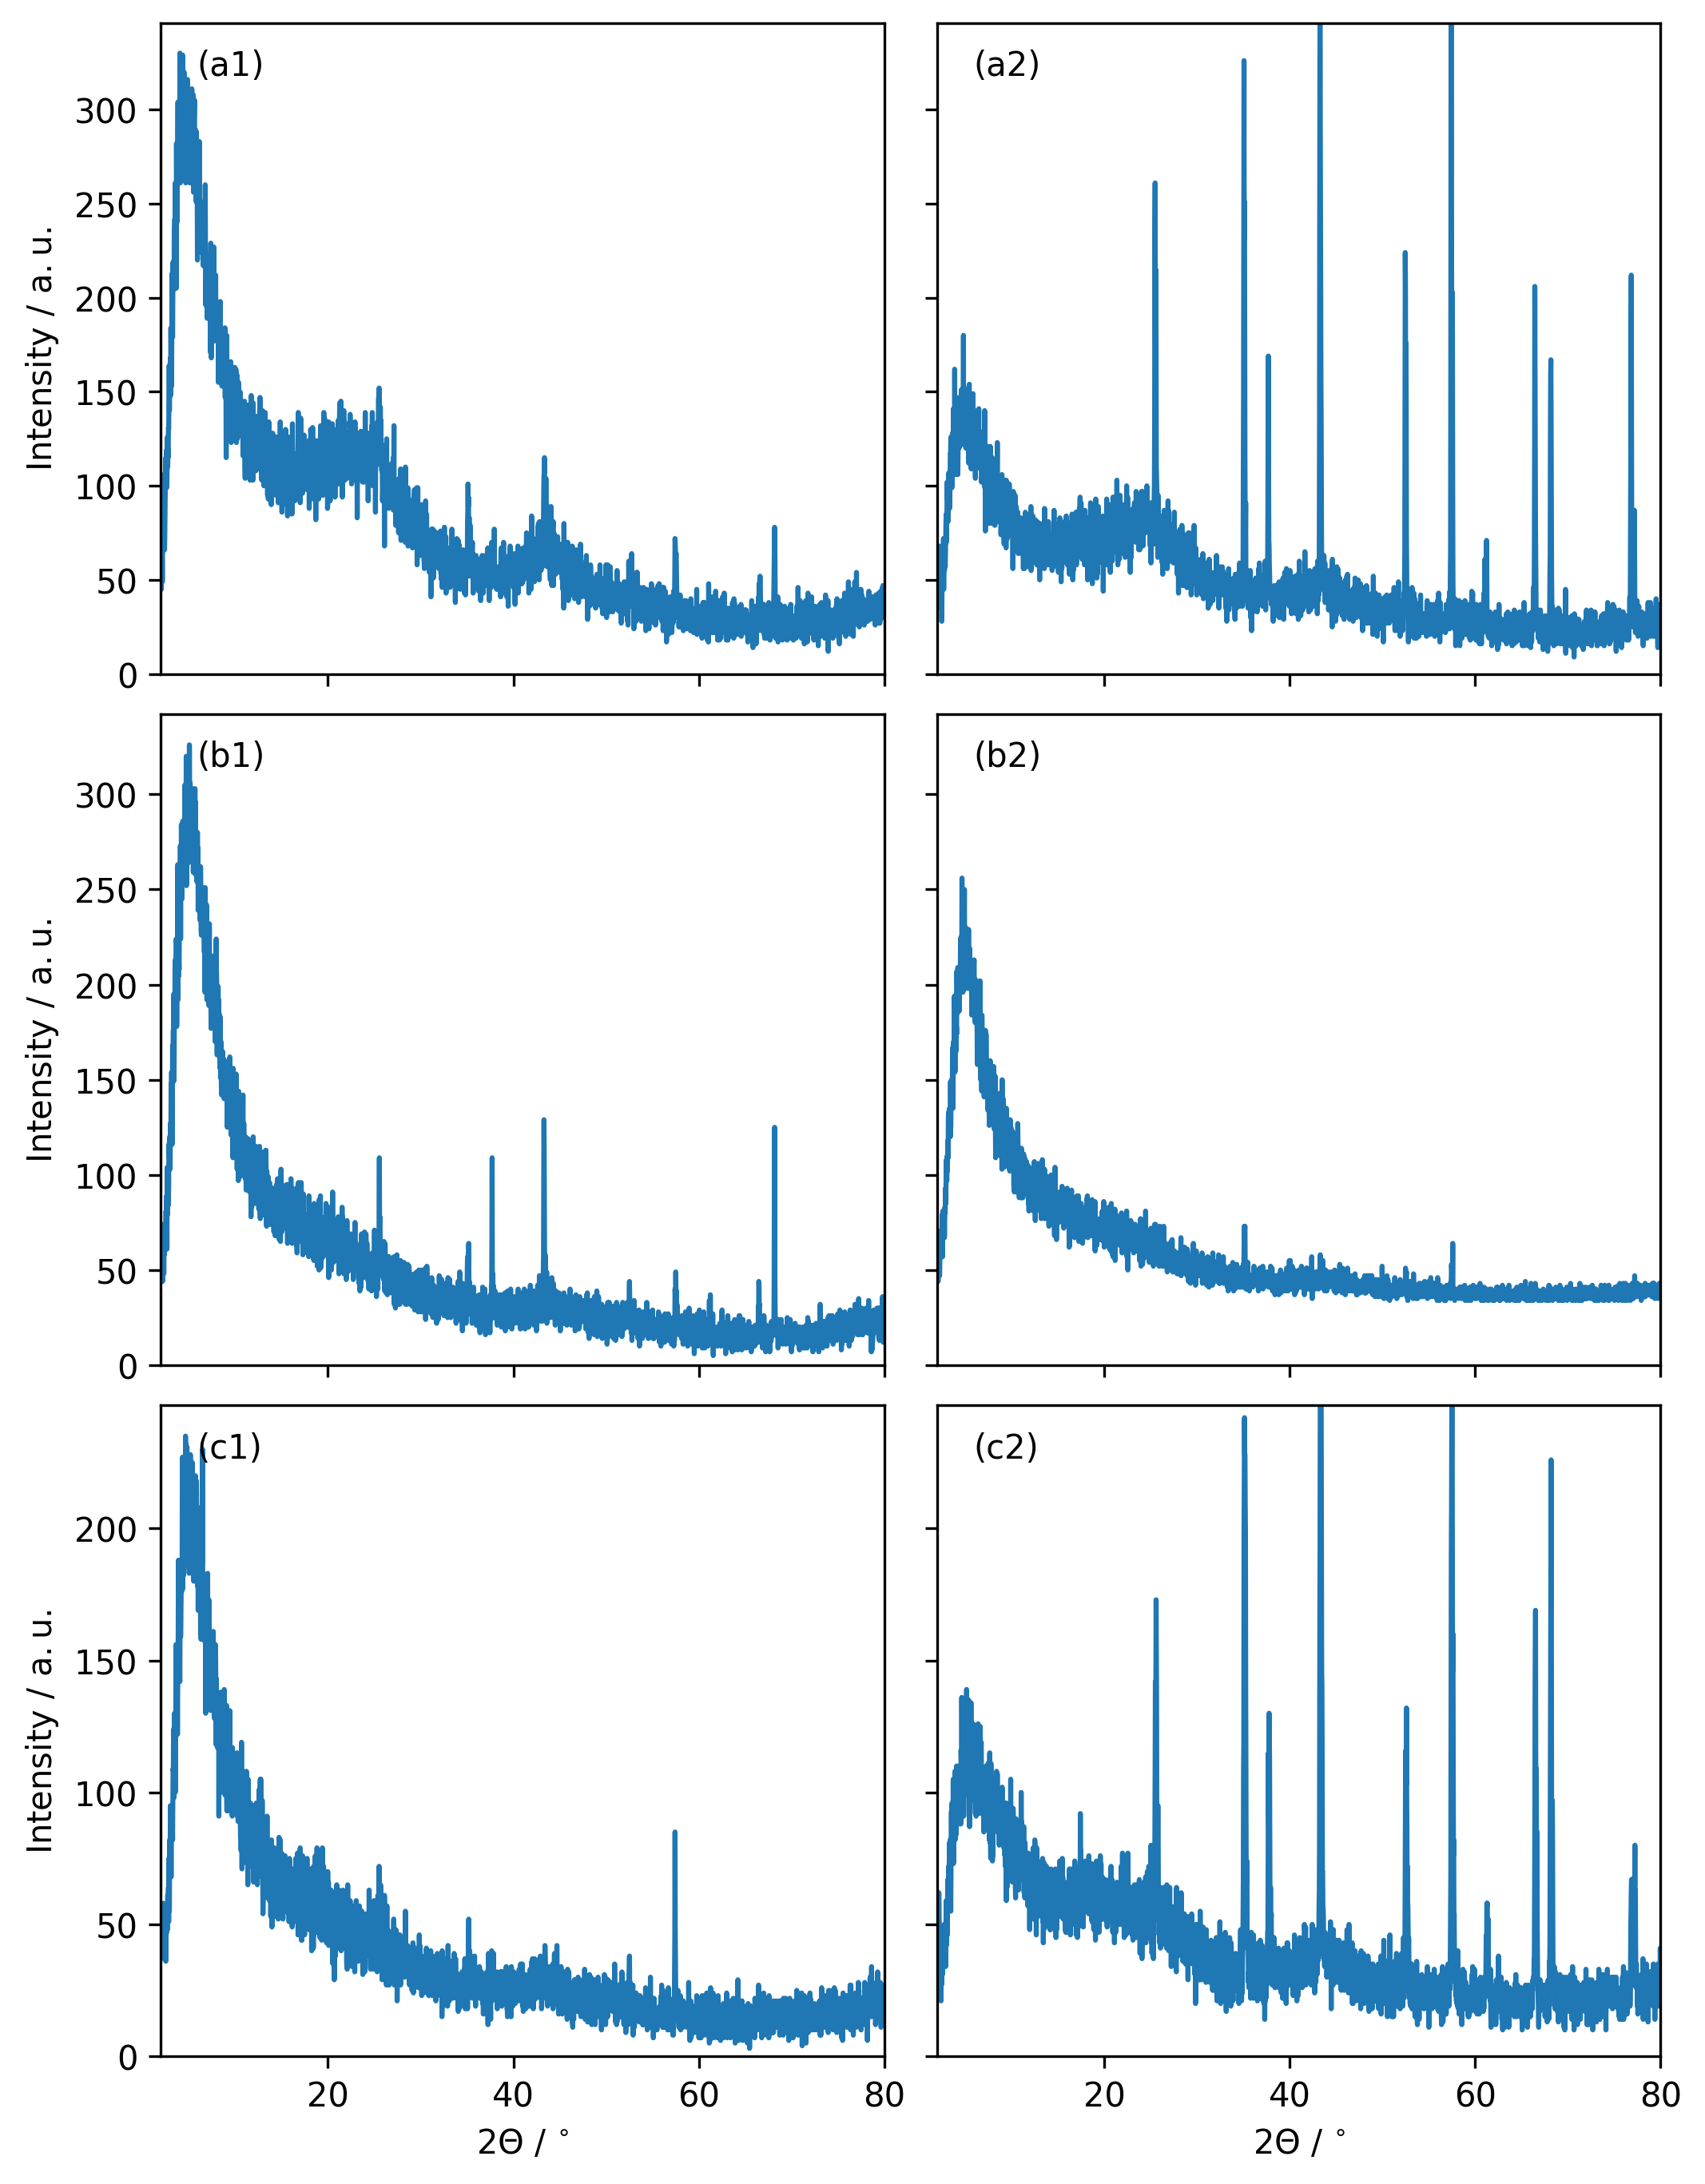
\includegraphics[width=\columnwidth, keepaspectratio]{4-cbs/figs/xrd_KOH.png}
    \caption{P-XRD spectra for samples hC-4600 (a1), hD-4600 (a2), hC-4700 (b1), hD-4700 (b2), hC-4800 (c1), hD-4800 (c2).}
    \label{fig:xrd_KOH}
\end{figure}

\begin{figure}[h]
    \centering
    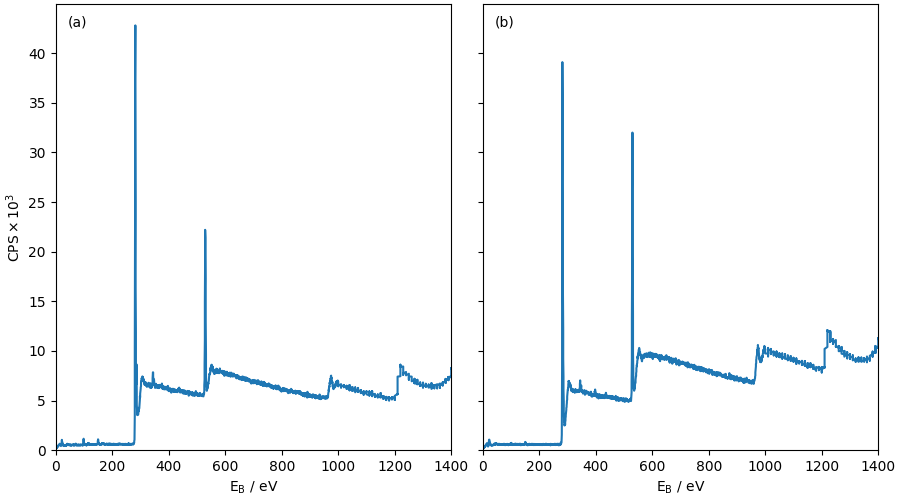
\includegraphics[width=\columnwidth, keepaspectratio]{4-cbs/figs/xps.png}
    \caption{XPS spectra for samples hD-0700 (a) and hD-hydrochar (b).}
    \label{fig:cb_xps}
\end{figure}

\begin{figure}[h!]
    \centering
    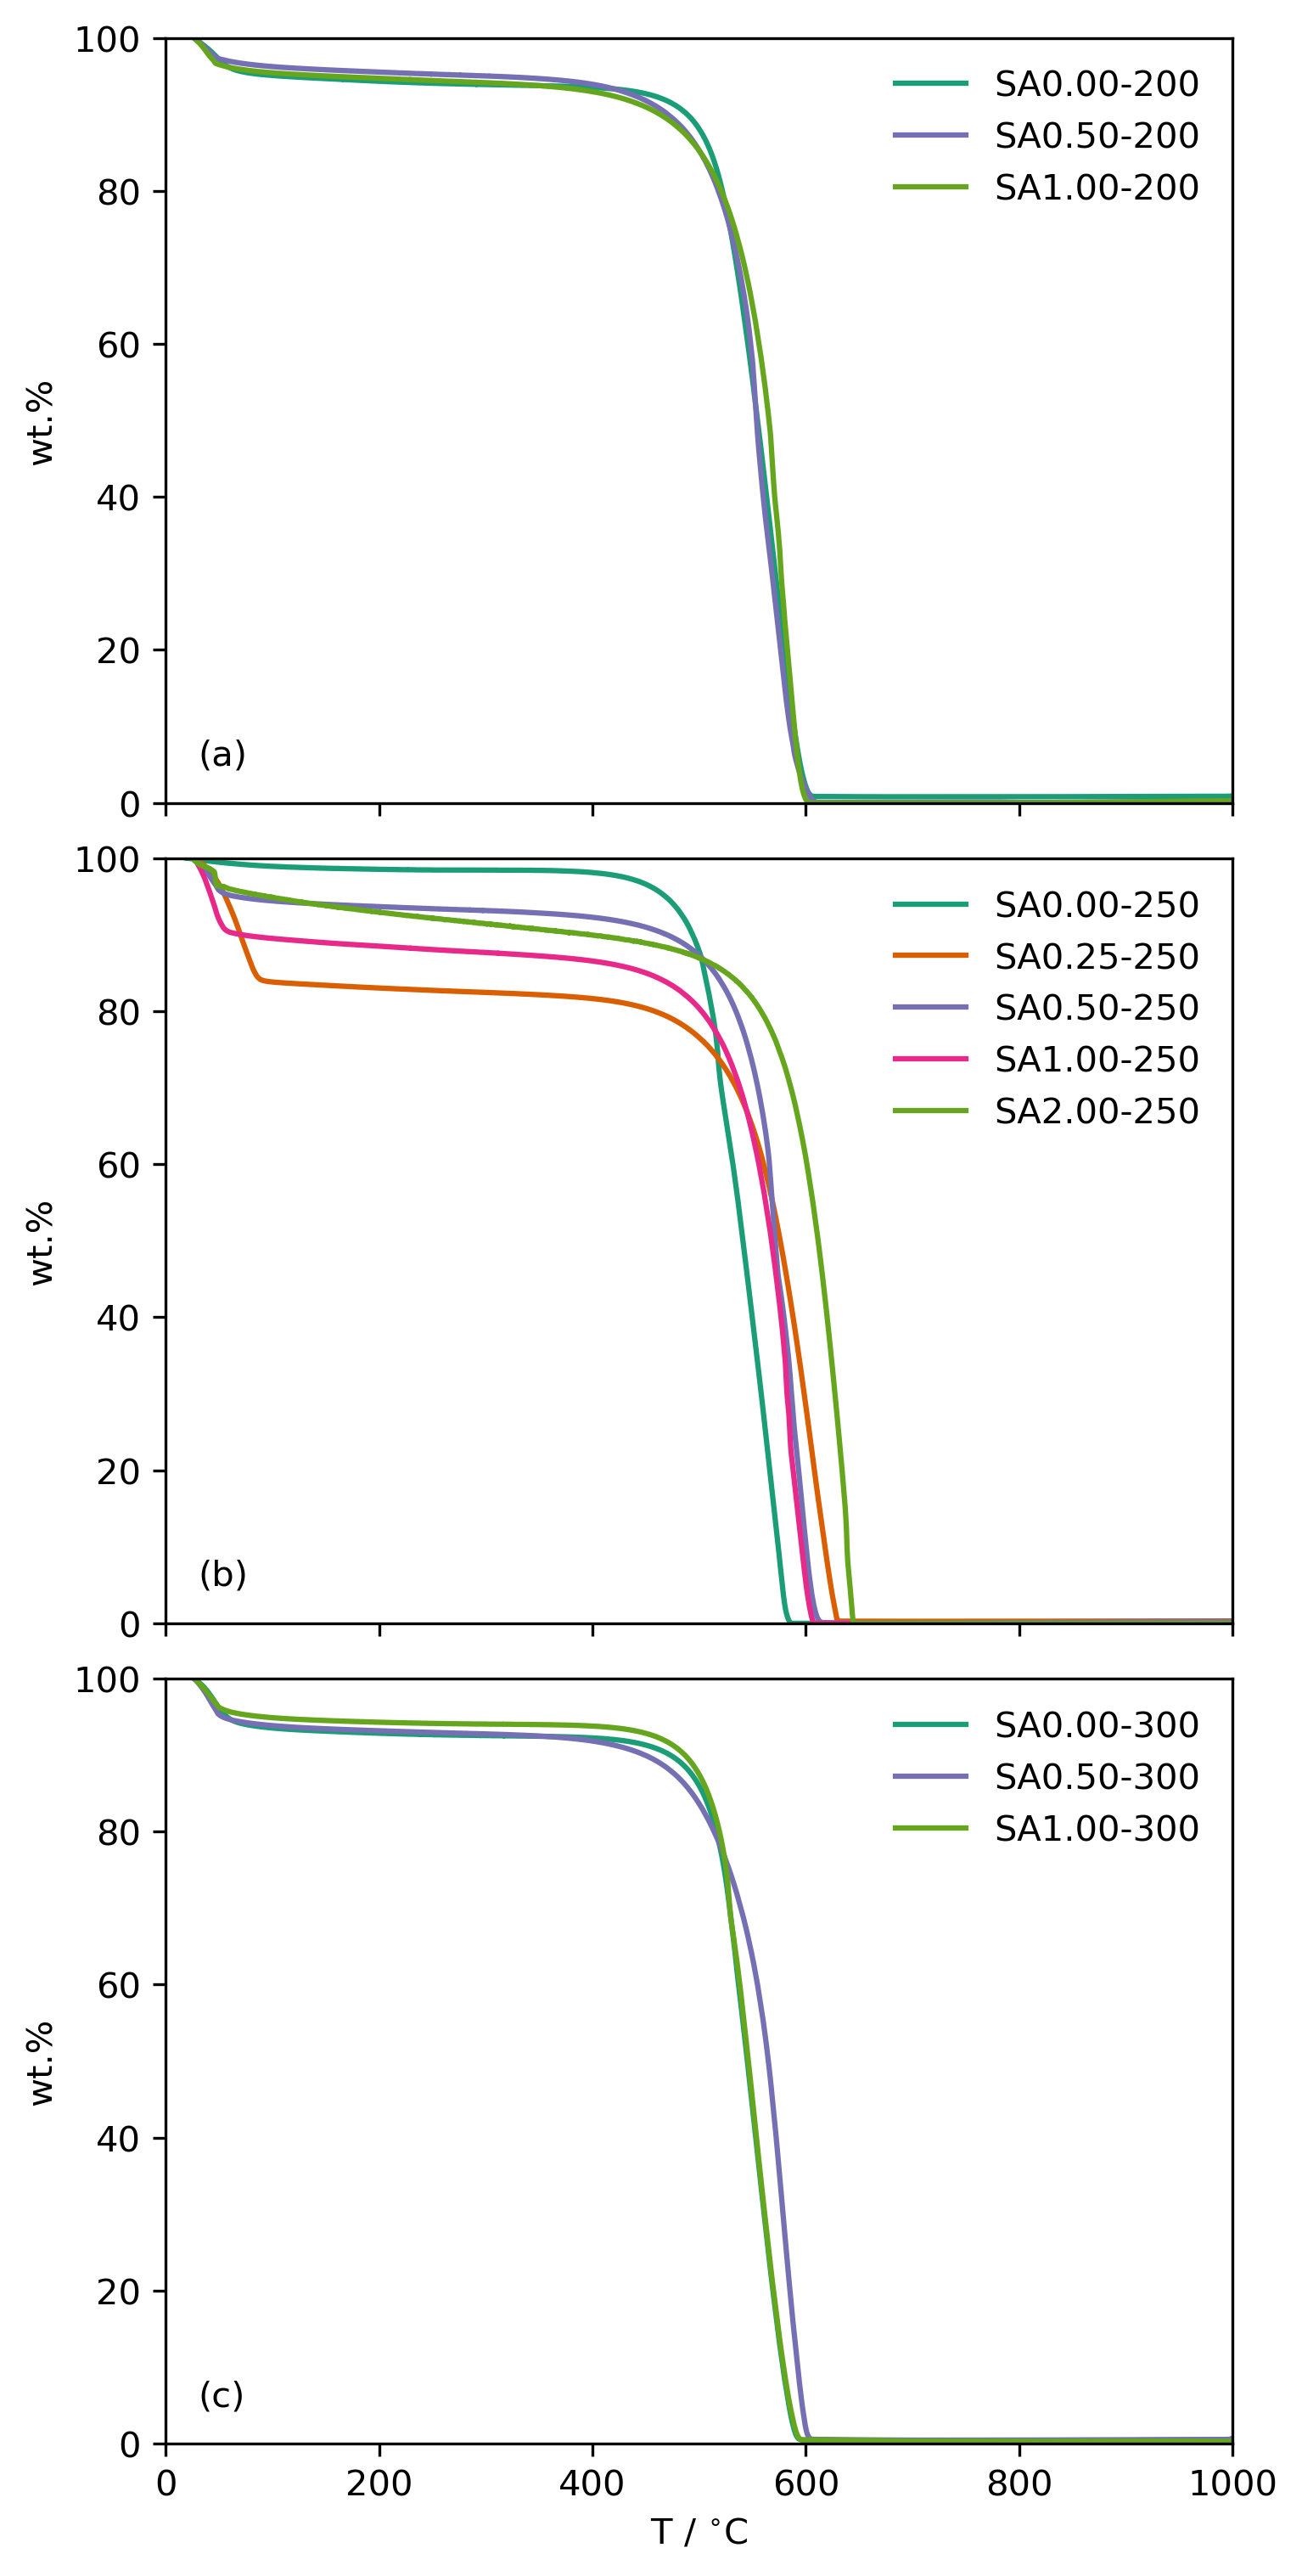
\includegraphics[width=0.8\columnwidth, keepaspectratio]{4-impregnation/figs/SD_tga_adj.png}
    \caption{TGA curves for SD\textit{x.xx-HHH} samples.}
    \label{fig:SD_tga}
\end{figure}

\chapter{Porosimetry}

\newpage
\begin{figure}[p]
    \centering
    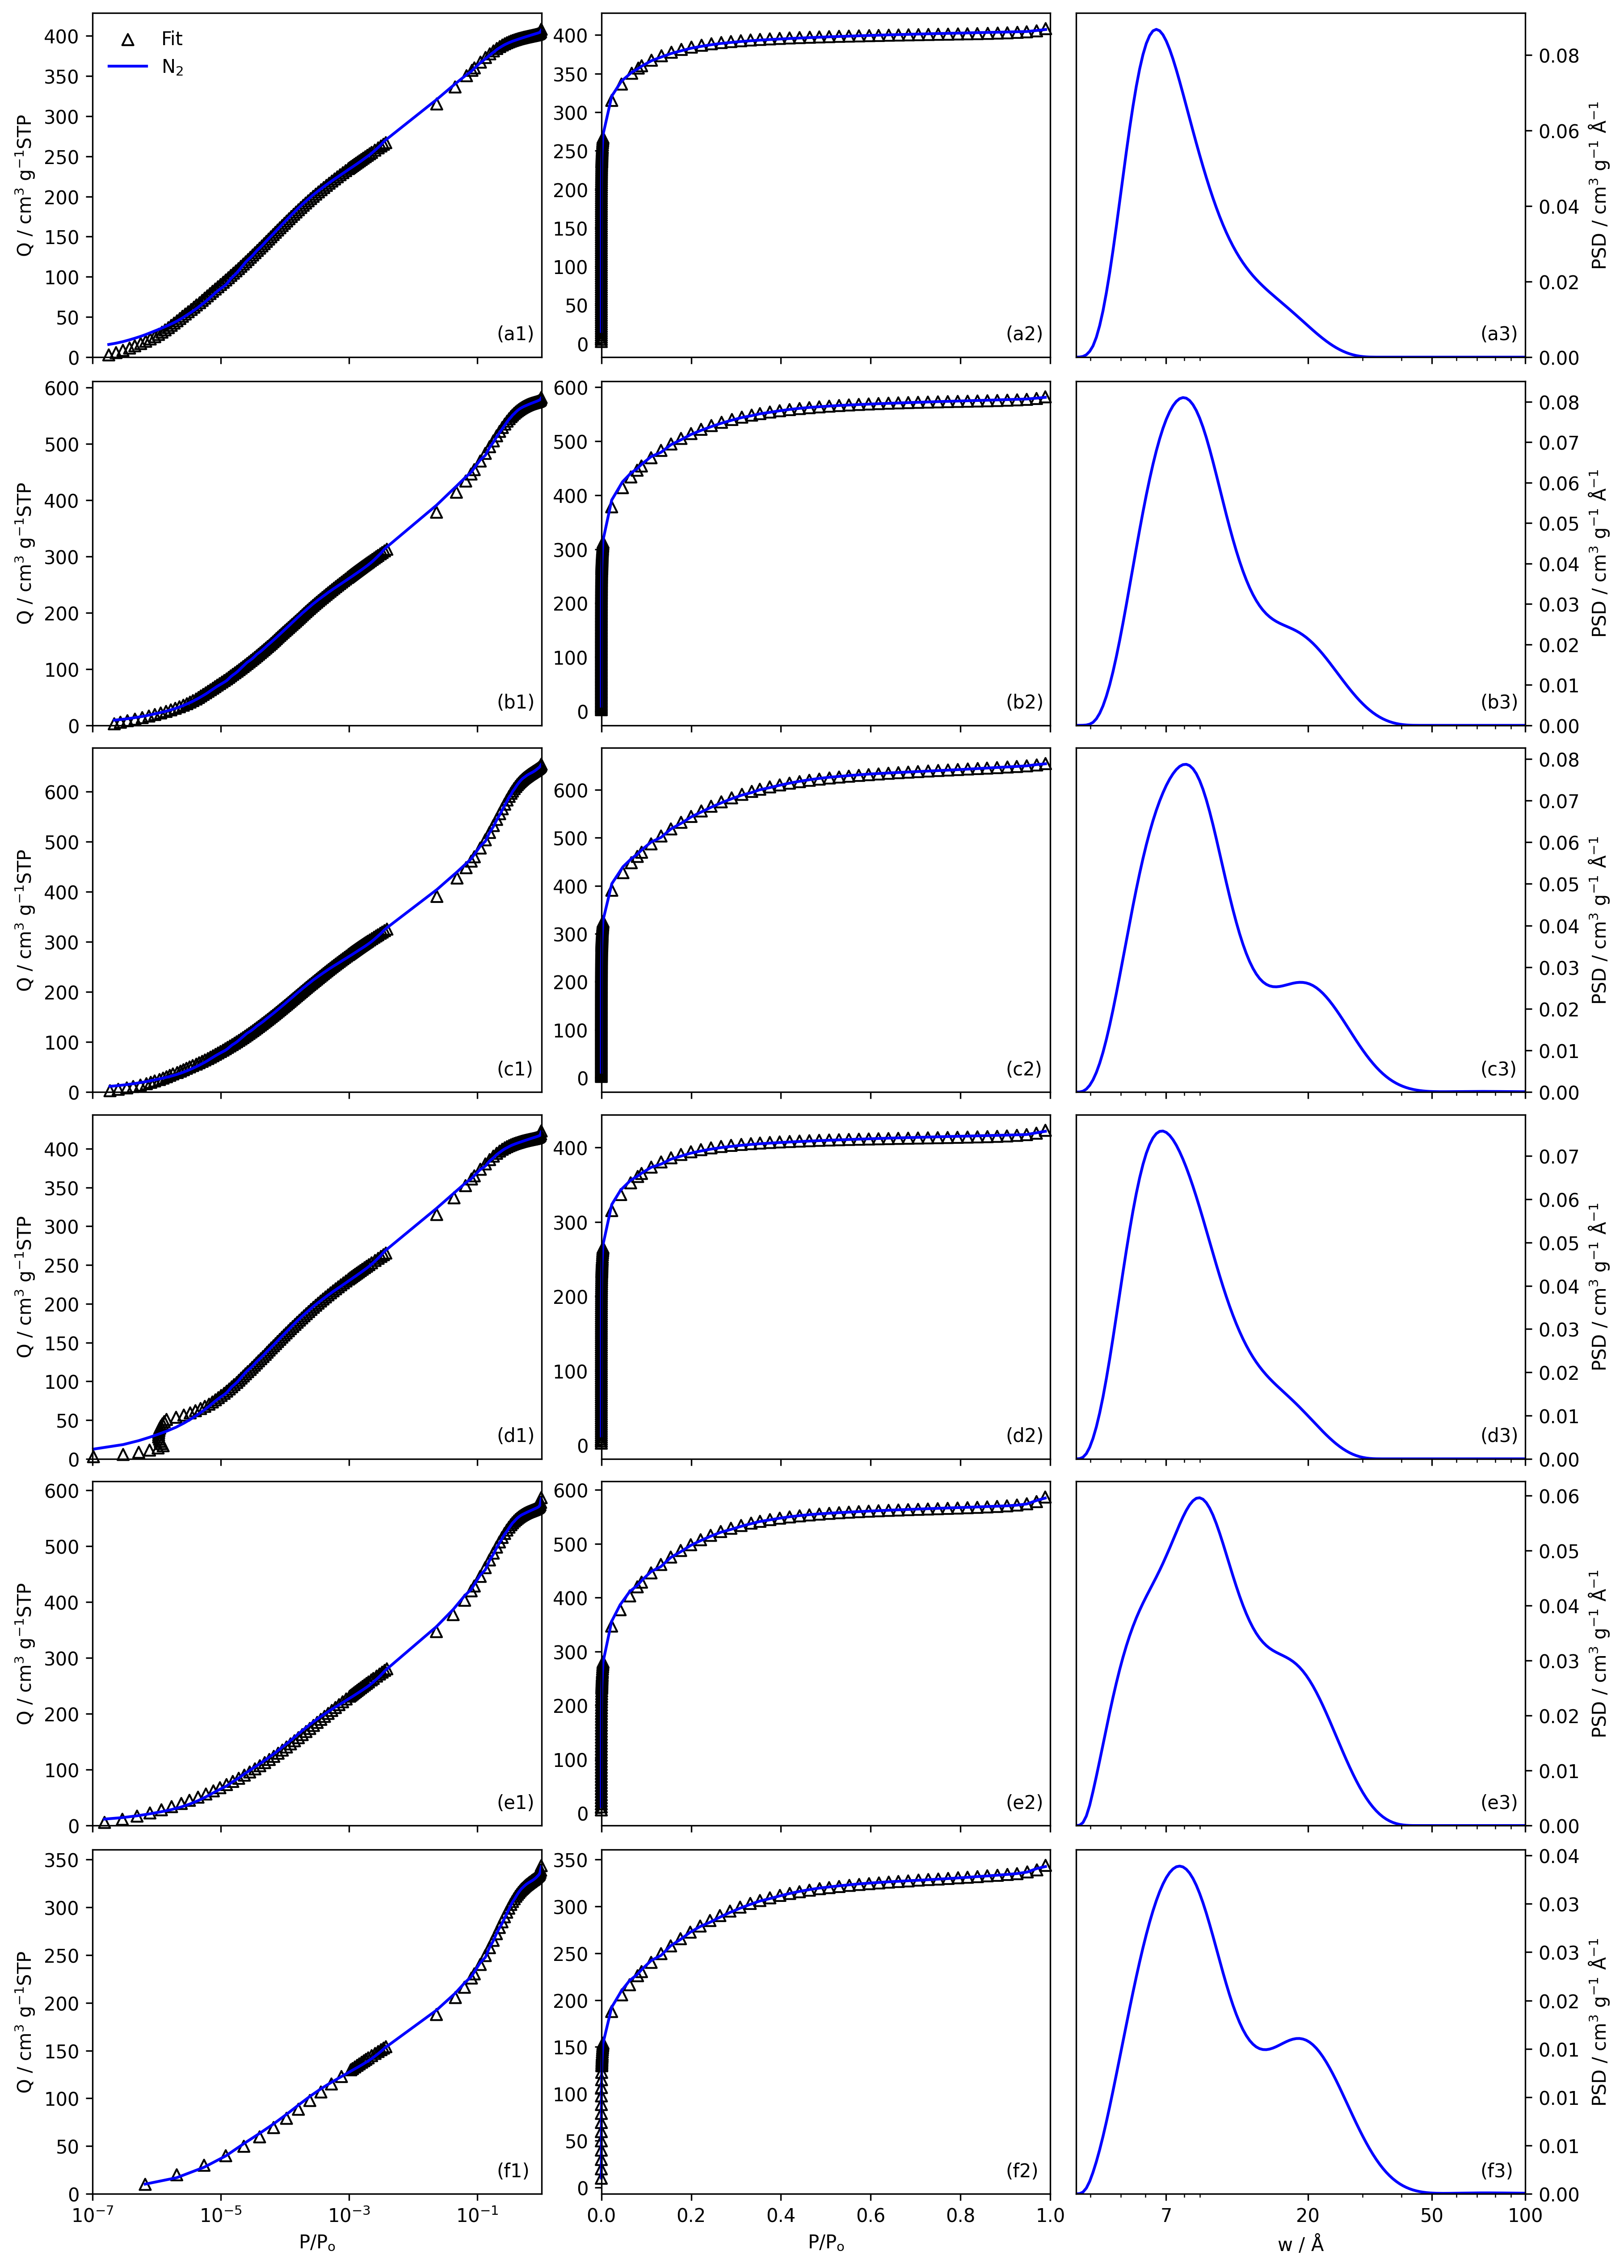
\includegraphics[width=\columnwidth, keepaspectratio]{4-cbs/figs/CB-4TTT_isopsd.png}
    \caption{Fits to \ce{N2} isotherms with logarithmic (a) and linear (b) relative pressure scale, and resultant differential PSDs (c) for samples hC-4600, hC-4700, hC-4800, hD-4600, hD-4700, hD-4800 in order in rows (1-6).}
    \label{fig:4TTT_psdisofull}
\end{figure}

\begin{figure}[p]
    \centering
    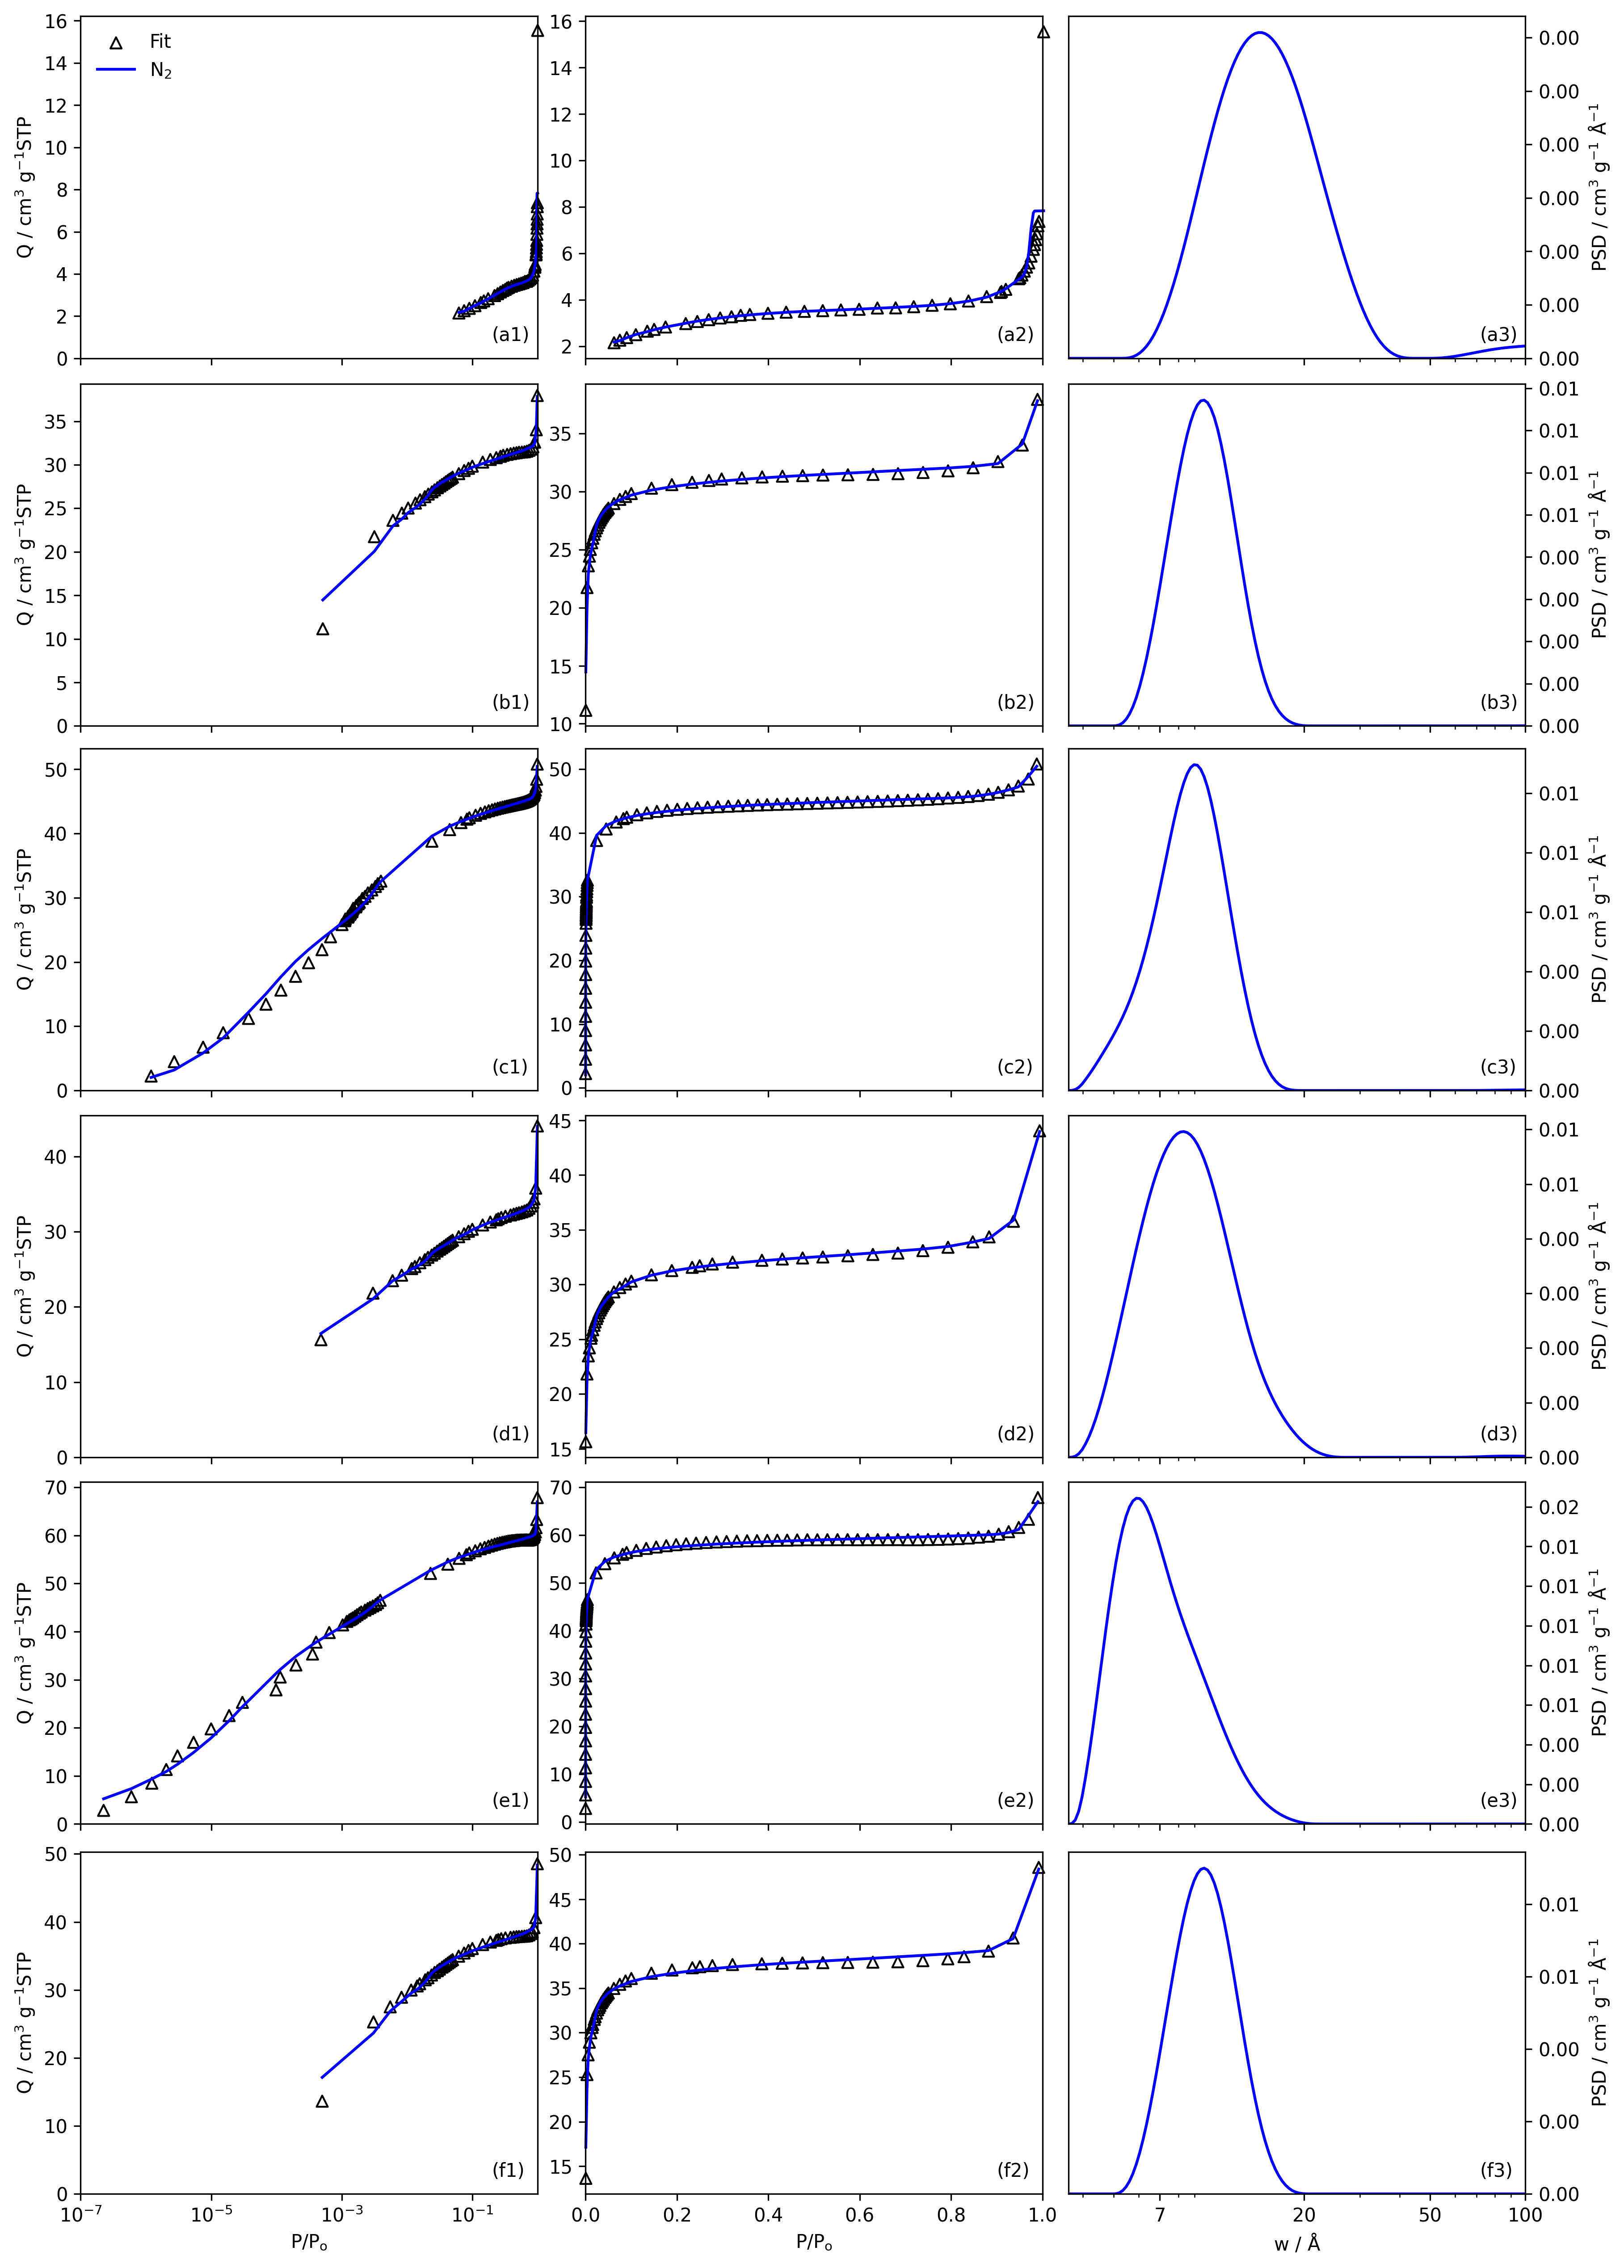
\includegraphics[width=\columnwidth, keepaspectratio]{4-cbs/figs/CB-0TTT_isopsd.png}
    \caption{Fits to \ce{N2} isotherms with logarithmic (a) and linear (b) relative pressure scale, and resultant differential PSDs (c) for samples hD-0600, hD-0700, hD-0800, hD-0600$'$, hD-0700$'$, and hD-0800$'$ in order in rows (1-6).}
    \label{fig:0TTT_psdisofull}
\end{figure}

\begin{figure}[h]
    \centering
    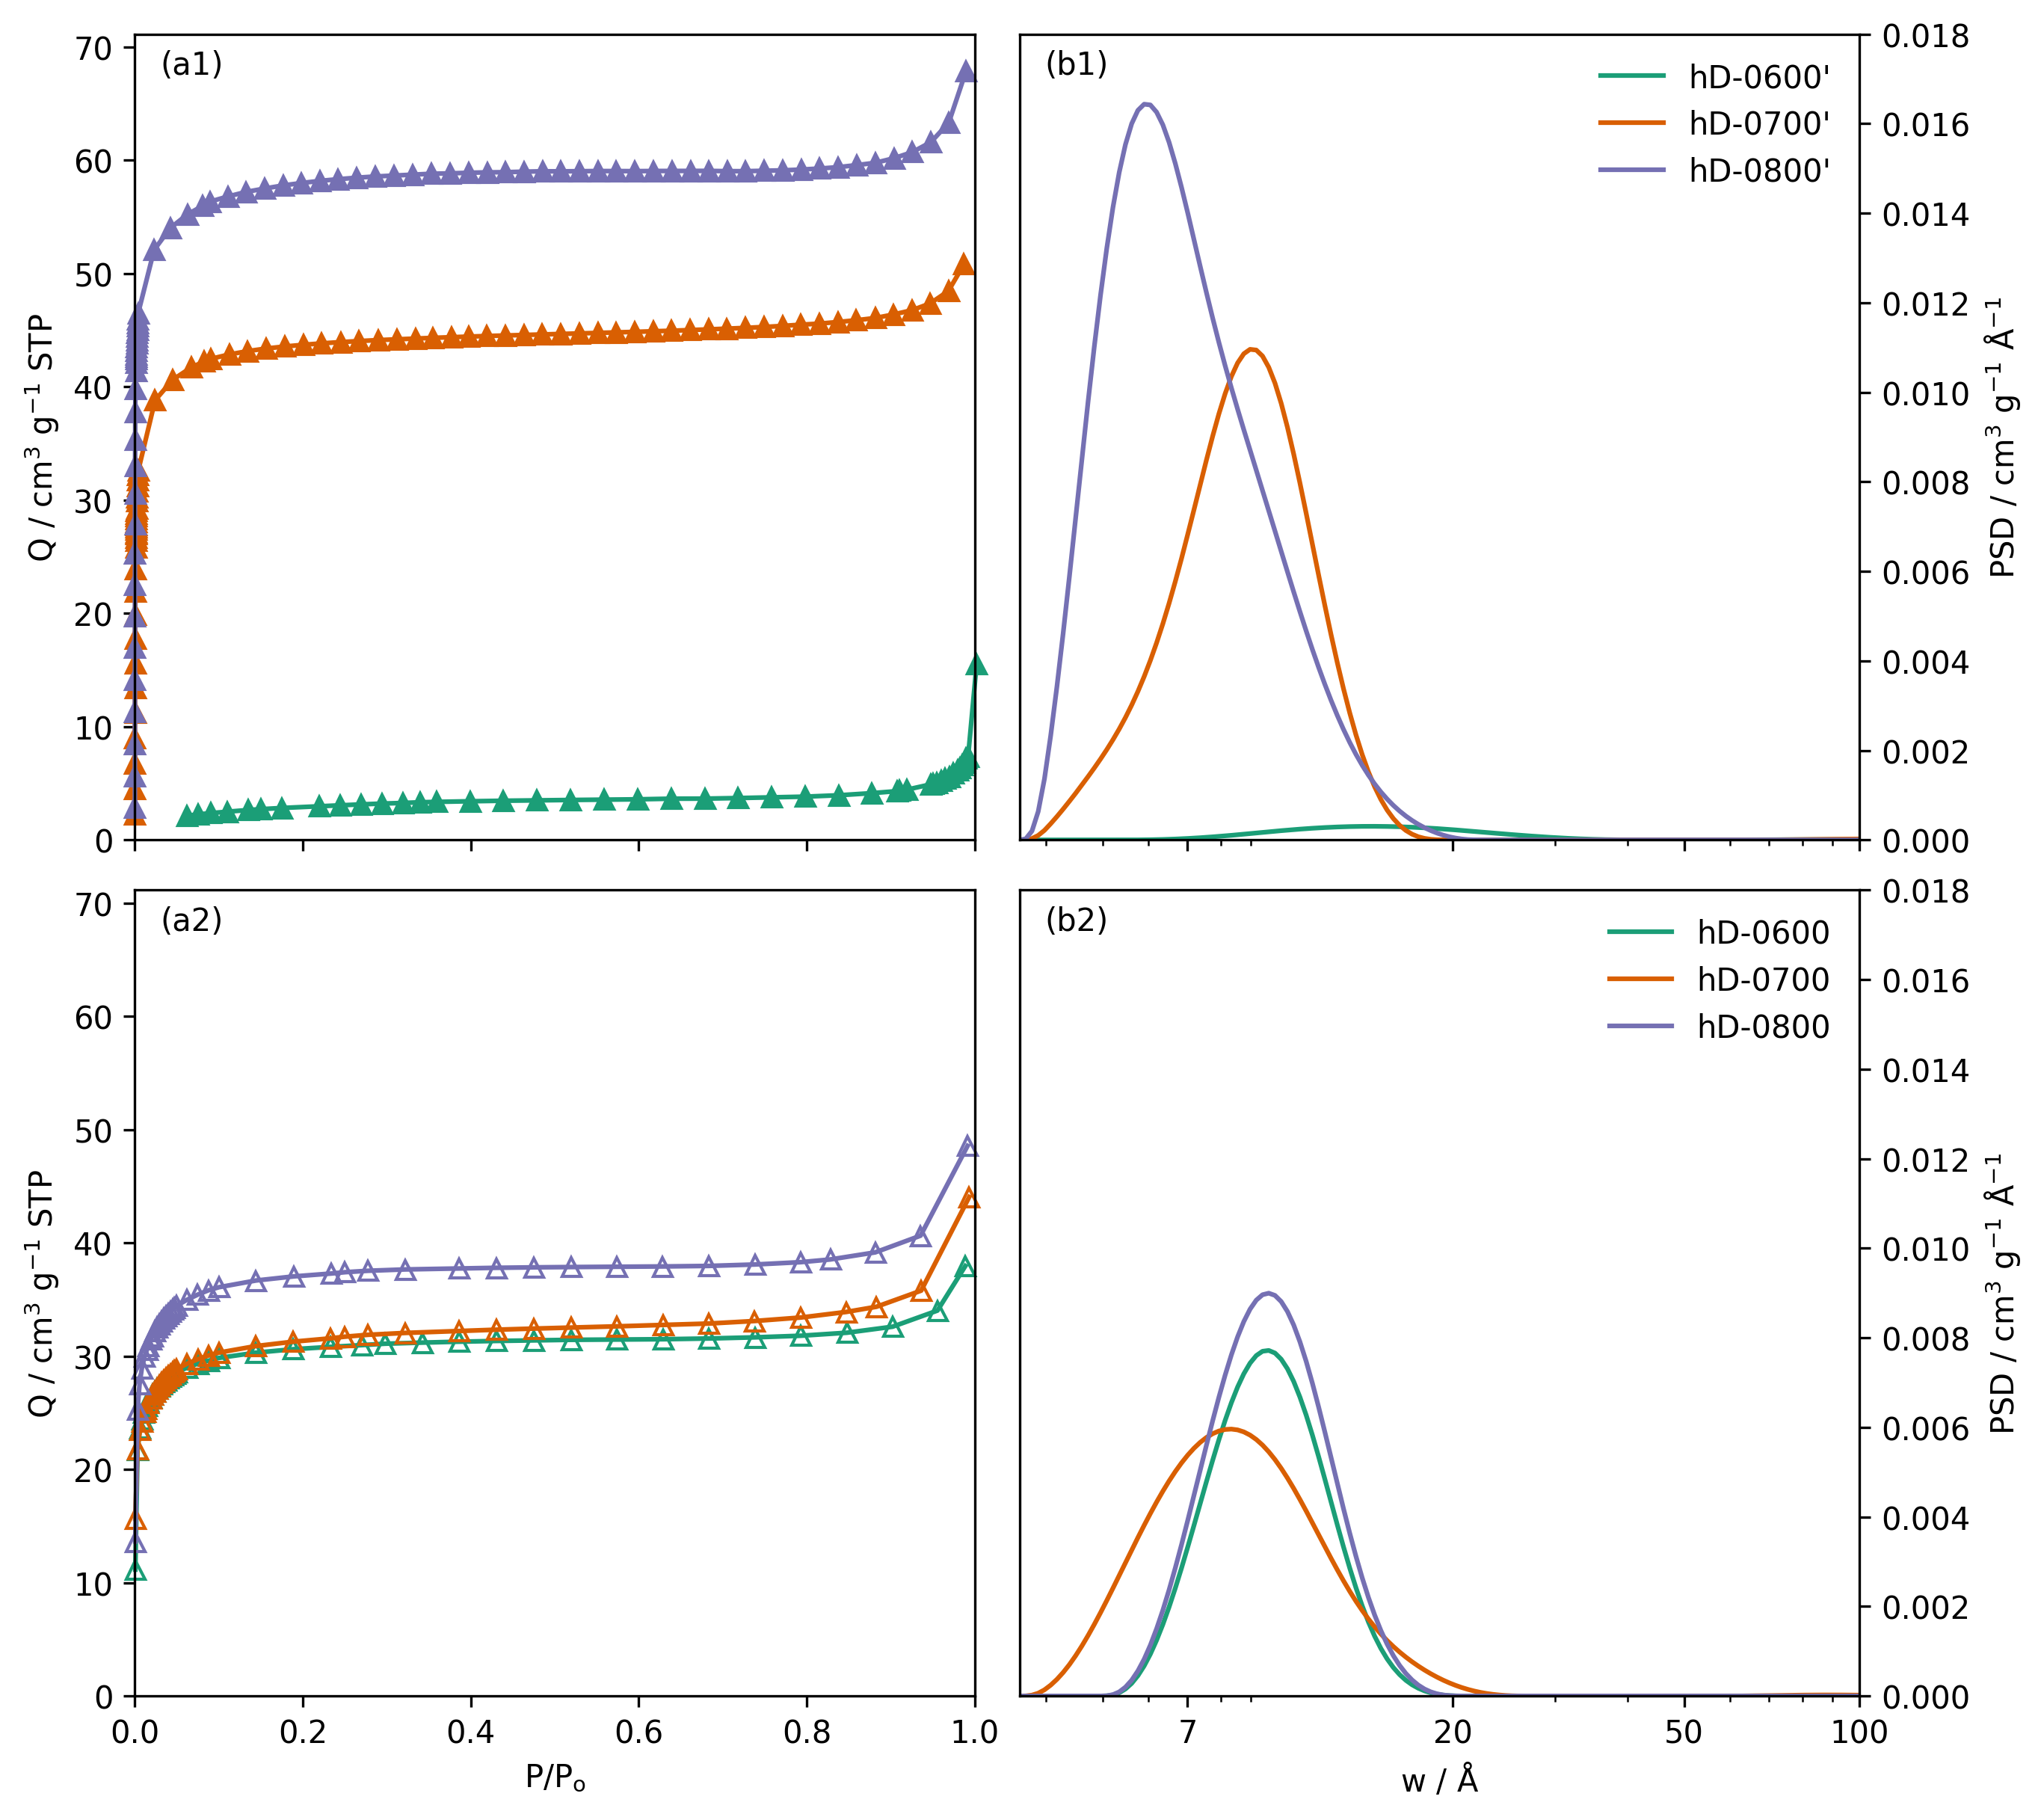
\includegraphics[width=\columnwidth, keepaspectratio]{4-cbs/figs/0TTT_n2_isotherms.png}
    \caption{Isotherms and resultant PSDs for samples hD-0\textit{TTT} and hD-0\textit{TTT}$'$.}
    \label{fig:0TTT_psdiso}
\end{figure}


\begin{figure}[h]
    \centering
    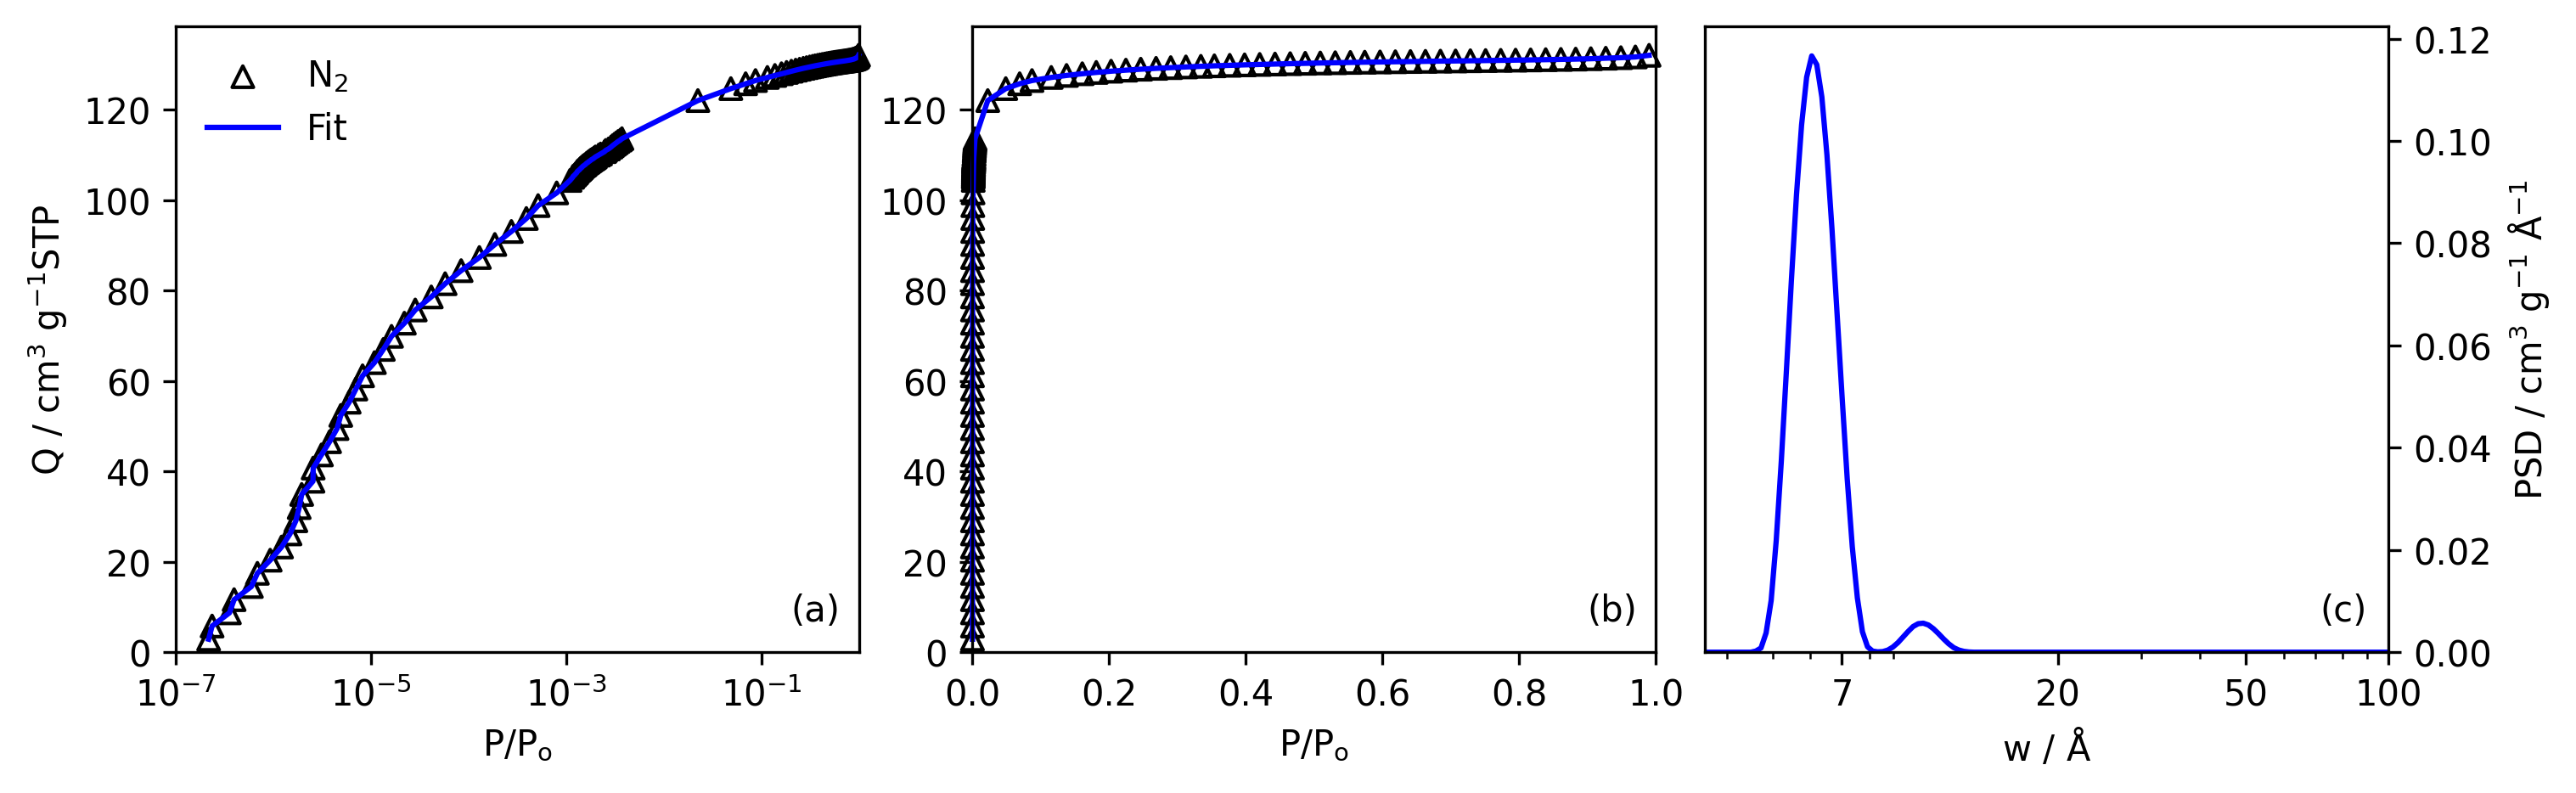
\includegraphics[width=\columnwidth, keepaspectratio]{4-cbs/figs/CA_iso_psd.png}
    \caption{Fits to \ce{N2} isotherms with logarithmic (a) and linear (b) relative pressure scale, and resultant differential PSDs (c) for the cellulose acetate derived sample CA-0800.}
    \label{fig:CA_psdiso}
\end{figure}

\clearpage
\begin{table}[h]
    \centering
    \caption{Porosity of CA-0800}
    \label{tb:CA_porosity}
    \begin{tabularx}{0.9\textwidth}{llllll}
    \toprule
        \multicolumn{2}{l}{$\mathbf{A_{BET}\ /\ m^2\ g^{-1}}$}  & \multicolumn{2}{l}{\textbf{Pore volume} / $\mathbf{cm^3\ g^{-1}}$} & \multicolumn{2}{l}{\textbf{Pore size / \AA}} \\
    \midrule
    522 & (491) & 0.20 & (0.19) & 6 \\
    \bottomrule
    \end{tabularx}
\end{table}

\begin{figure}[p]
    \centering
    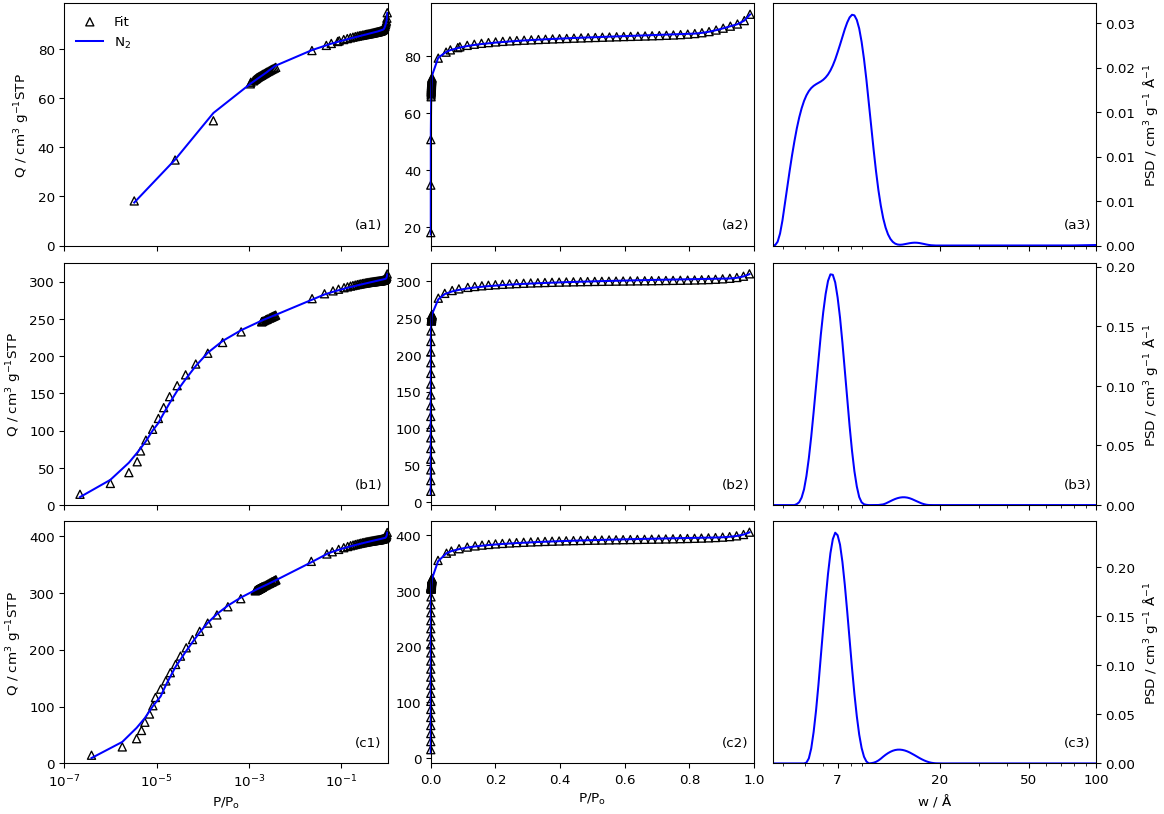
\includegraphics[width=\columnwidth, keepaspectratio]{4-impregnation/figs/SAxxx-200_isopsd.png}
    \caption{Fits to \ce{N2} isotherms with logarithmic (a) and linear (b) relative pressure scale, and resultant differential PSDs (c) for samples SA0.00-200, SA0.50-200, and SA1.00-200 in order in rows (1-3).}
    \label{fig:SAxxx-200_isopsd}
\end{figure}

\begin{figure}[p]
    \centering
    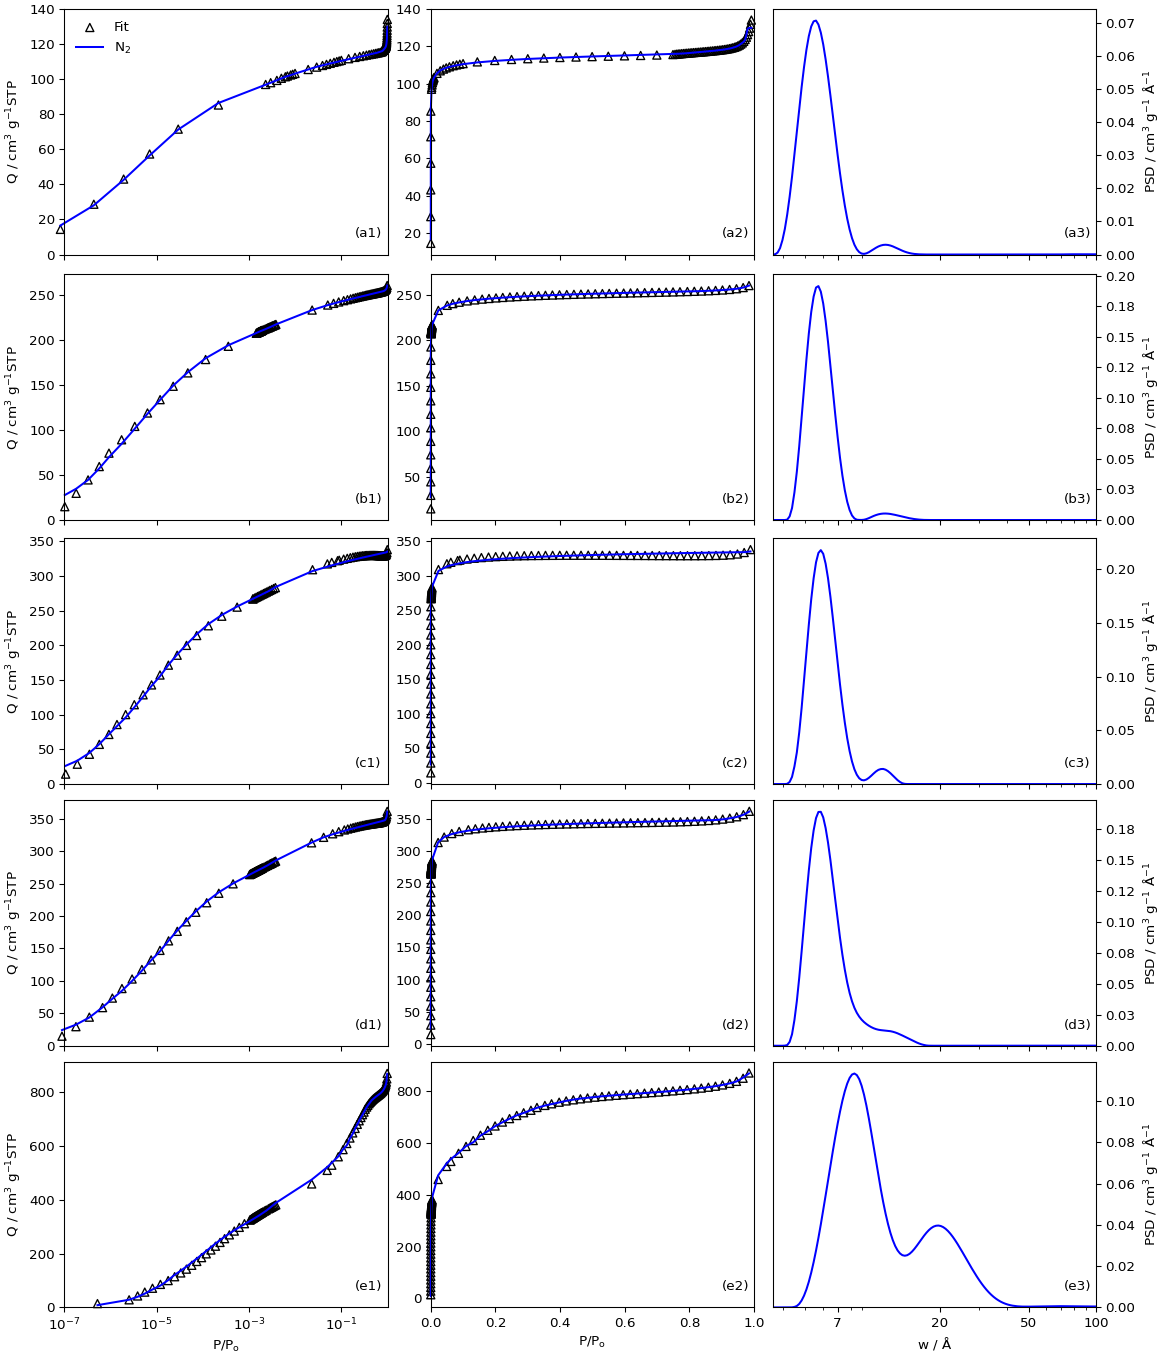
\includegraphics[width=\columnwidth, keepaspectratio]{4-impregnation/figs/SAxxx-250_isopsd.png}
    \caption{Fits to \ce{N2} isotherms with logarithmic (a) and linear (b) relative pressure scale, and resultant differential PSDs (c) for samples SA0.00-250, SA0.25-250, SA0.50-250, SA1.0-250, and SA2.00-250 in order in rows (1-5).}
    \label{fig:SAxxx-250_isopsd}
\end{figure}

\begin{figure}[p]
    \centering
    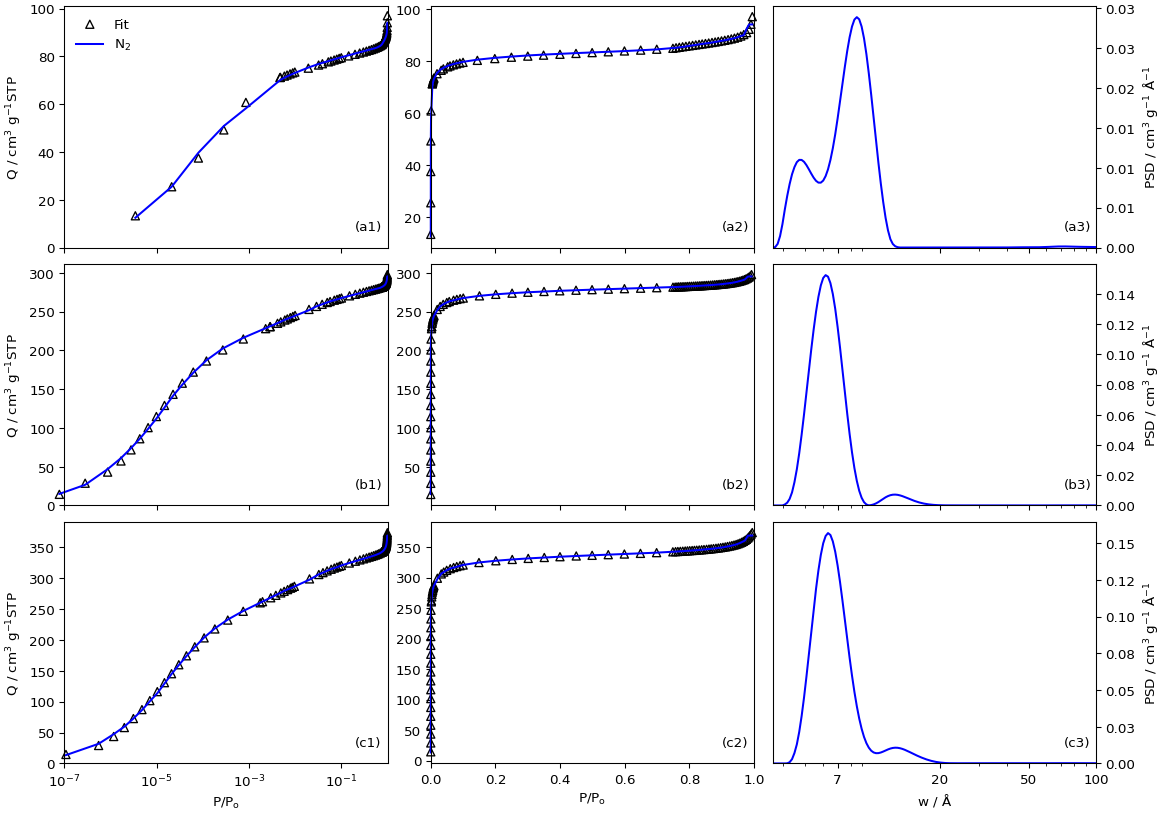
\includegraphics[width=\columnwidth, keepaspectratio]{4-impregnation/figs/SAxxx-300_isopsd.png}
    \caption{Fits to \ce{N2} isotherms with logarithmic (a) and linear (b) relative pressure scale, and resultant differential PSDs (c) for samples SA0.00-300, SA0.50-300, and SA1.00-300 in order in rows (1-3).}
    \label{fig:SAxxx-300_isopsd}
\end{figure}

\begin{figure}[p]
    \centering
    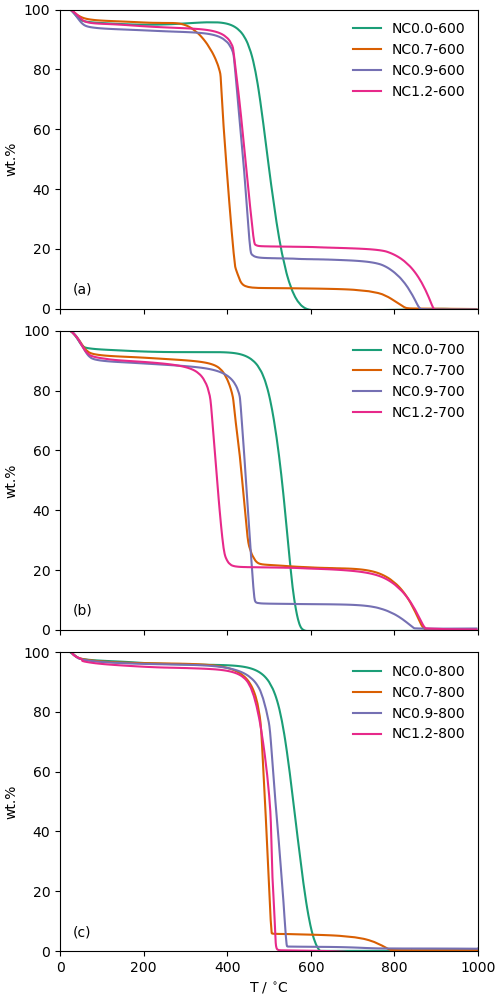
\includegraphics[width=0.87\columnwidth, keepaspectratio]{4-impregnation/figs/NC_tga.png}
    \caption{Unadjusted TGA curves for NC\textit{x.x-TTT} samples.}
    \label{fig:NC_tga}
\end{figure}

\begin{figure}[p]
    \centering
    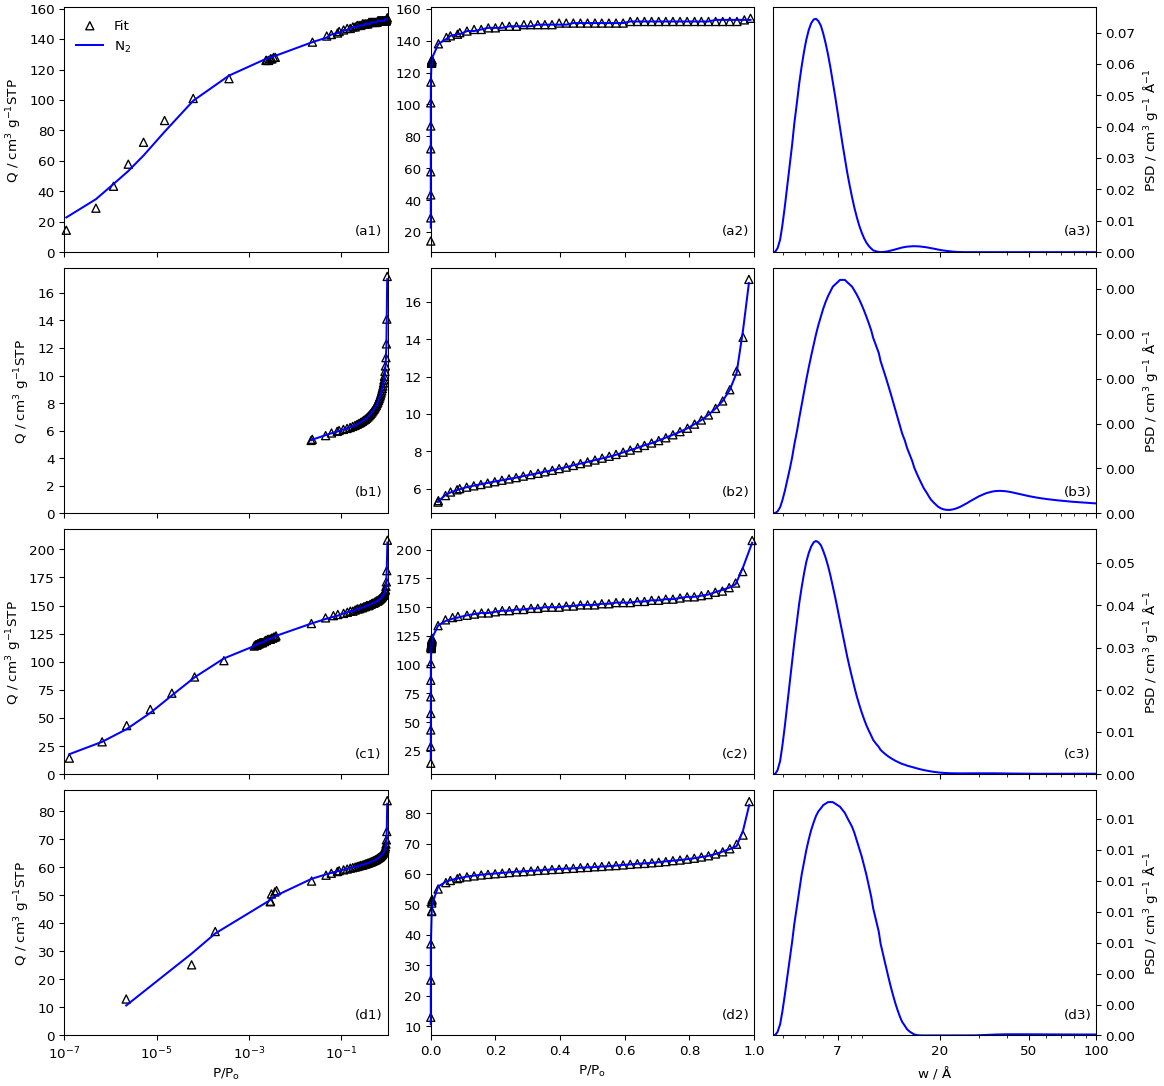
\includegraphics[width=\columnwidth, keepaspectratio]{4-impregnation/figs/NCxx-600_isopsd.png}
    \caption{Fits to \ce{N2} isotherms with logarithmic (a) and linear (b) relative pressure scale, and resultant differential PSDs (c) for samples NC0.0-600, NC0.7-600, NC0.9-600, and NC1.2-600 in order in rows (1-4).}
    \label{fig:NCxx-600_psdisofull}
\end{figure}

\begin{figure}[p]
    \centering
    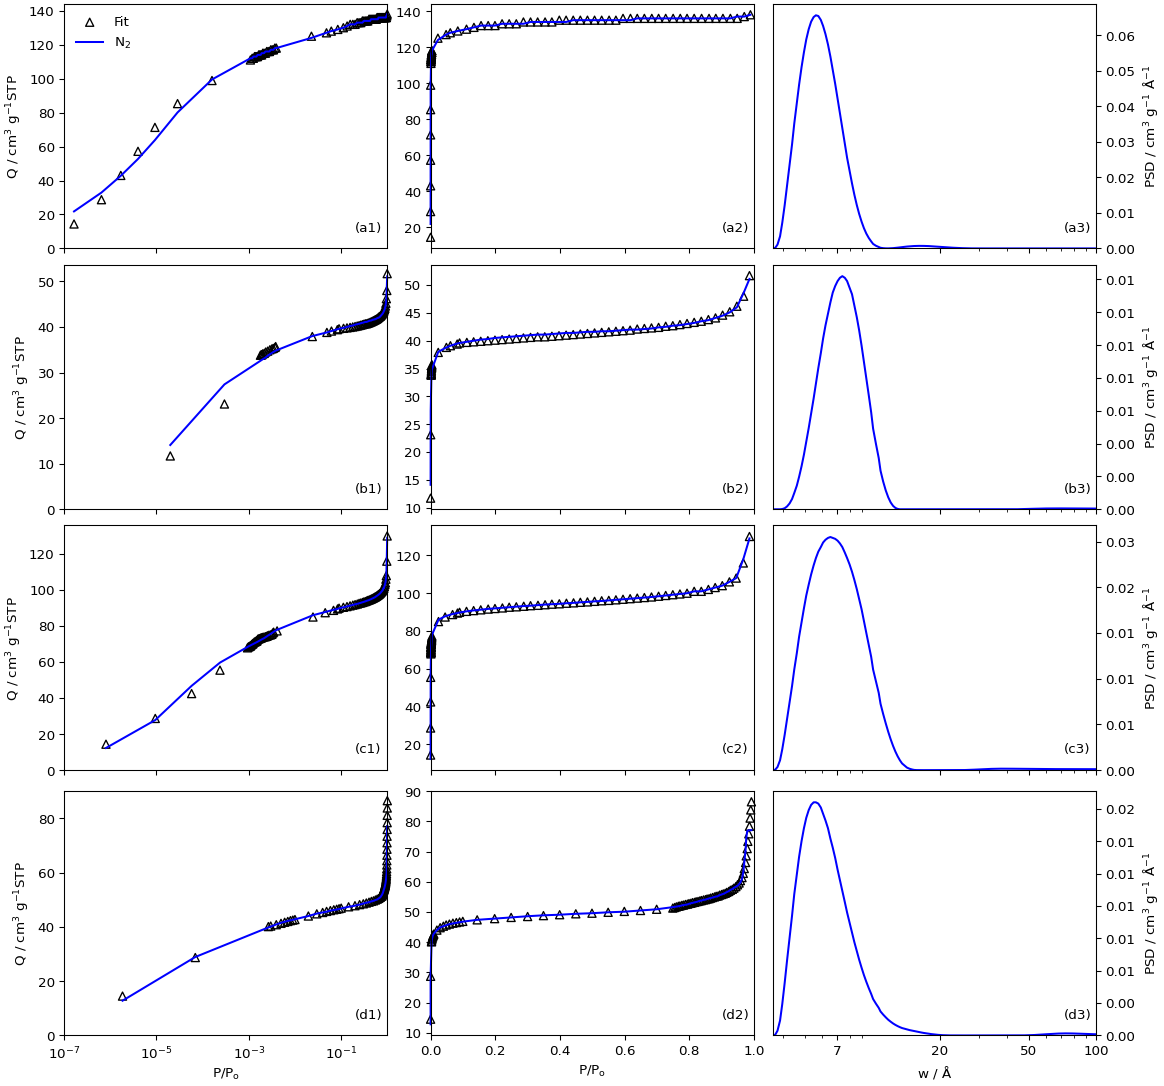
\includegraphics[width=\columnwidth, keepaspectratio]{4-impregnation/figs/NCxx-700_isopsd.png}
    \caption{Fits to \ce{N2} isotherms with logarithmic (a) and linear (b) relative pressure scale, and resultant differential PSDs (c) for samples NC0.0-700, NC0.7-700, NC0.9-700, and NC1.2-700 in order in rows (1-4).}
    \label{fig:NCxx-700_psdisofull}
\end{figure}

\begin{figure}[p]
    \centering
    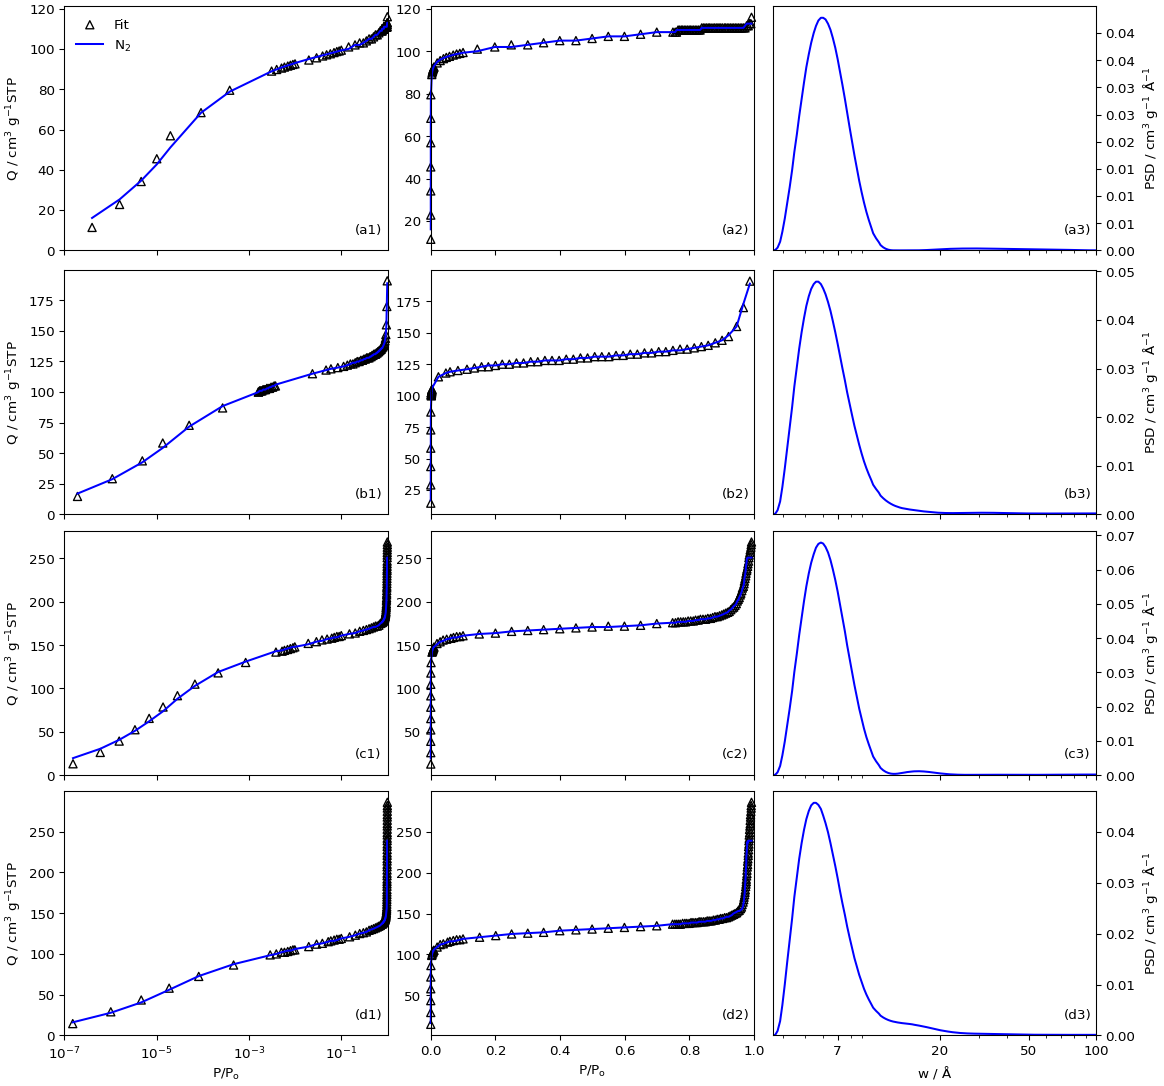
\includegraphics[width=\columnwidth, keepaspectratio]{4-impregnation/figs/NCxx-800_isopsd.png}
    \caption{Fits to \ce{N2} isotherms with logarithmic (a) and linear (b) relative pressure scale, and resultant differential PSDs (c) for samples NC0.0-800, NC0.7-800, NC0.9-800, and NC1.2-800 in order in rows (1-4).}
    \label{fig:NCxx-800_psdisofull}
\end{figure}

\begin{figure}[p]
    \centering
    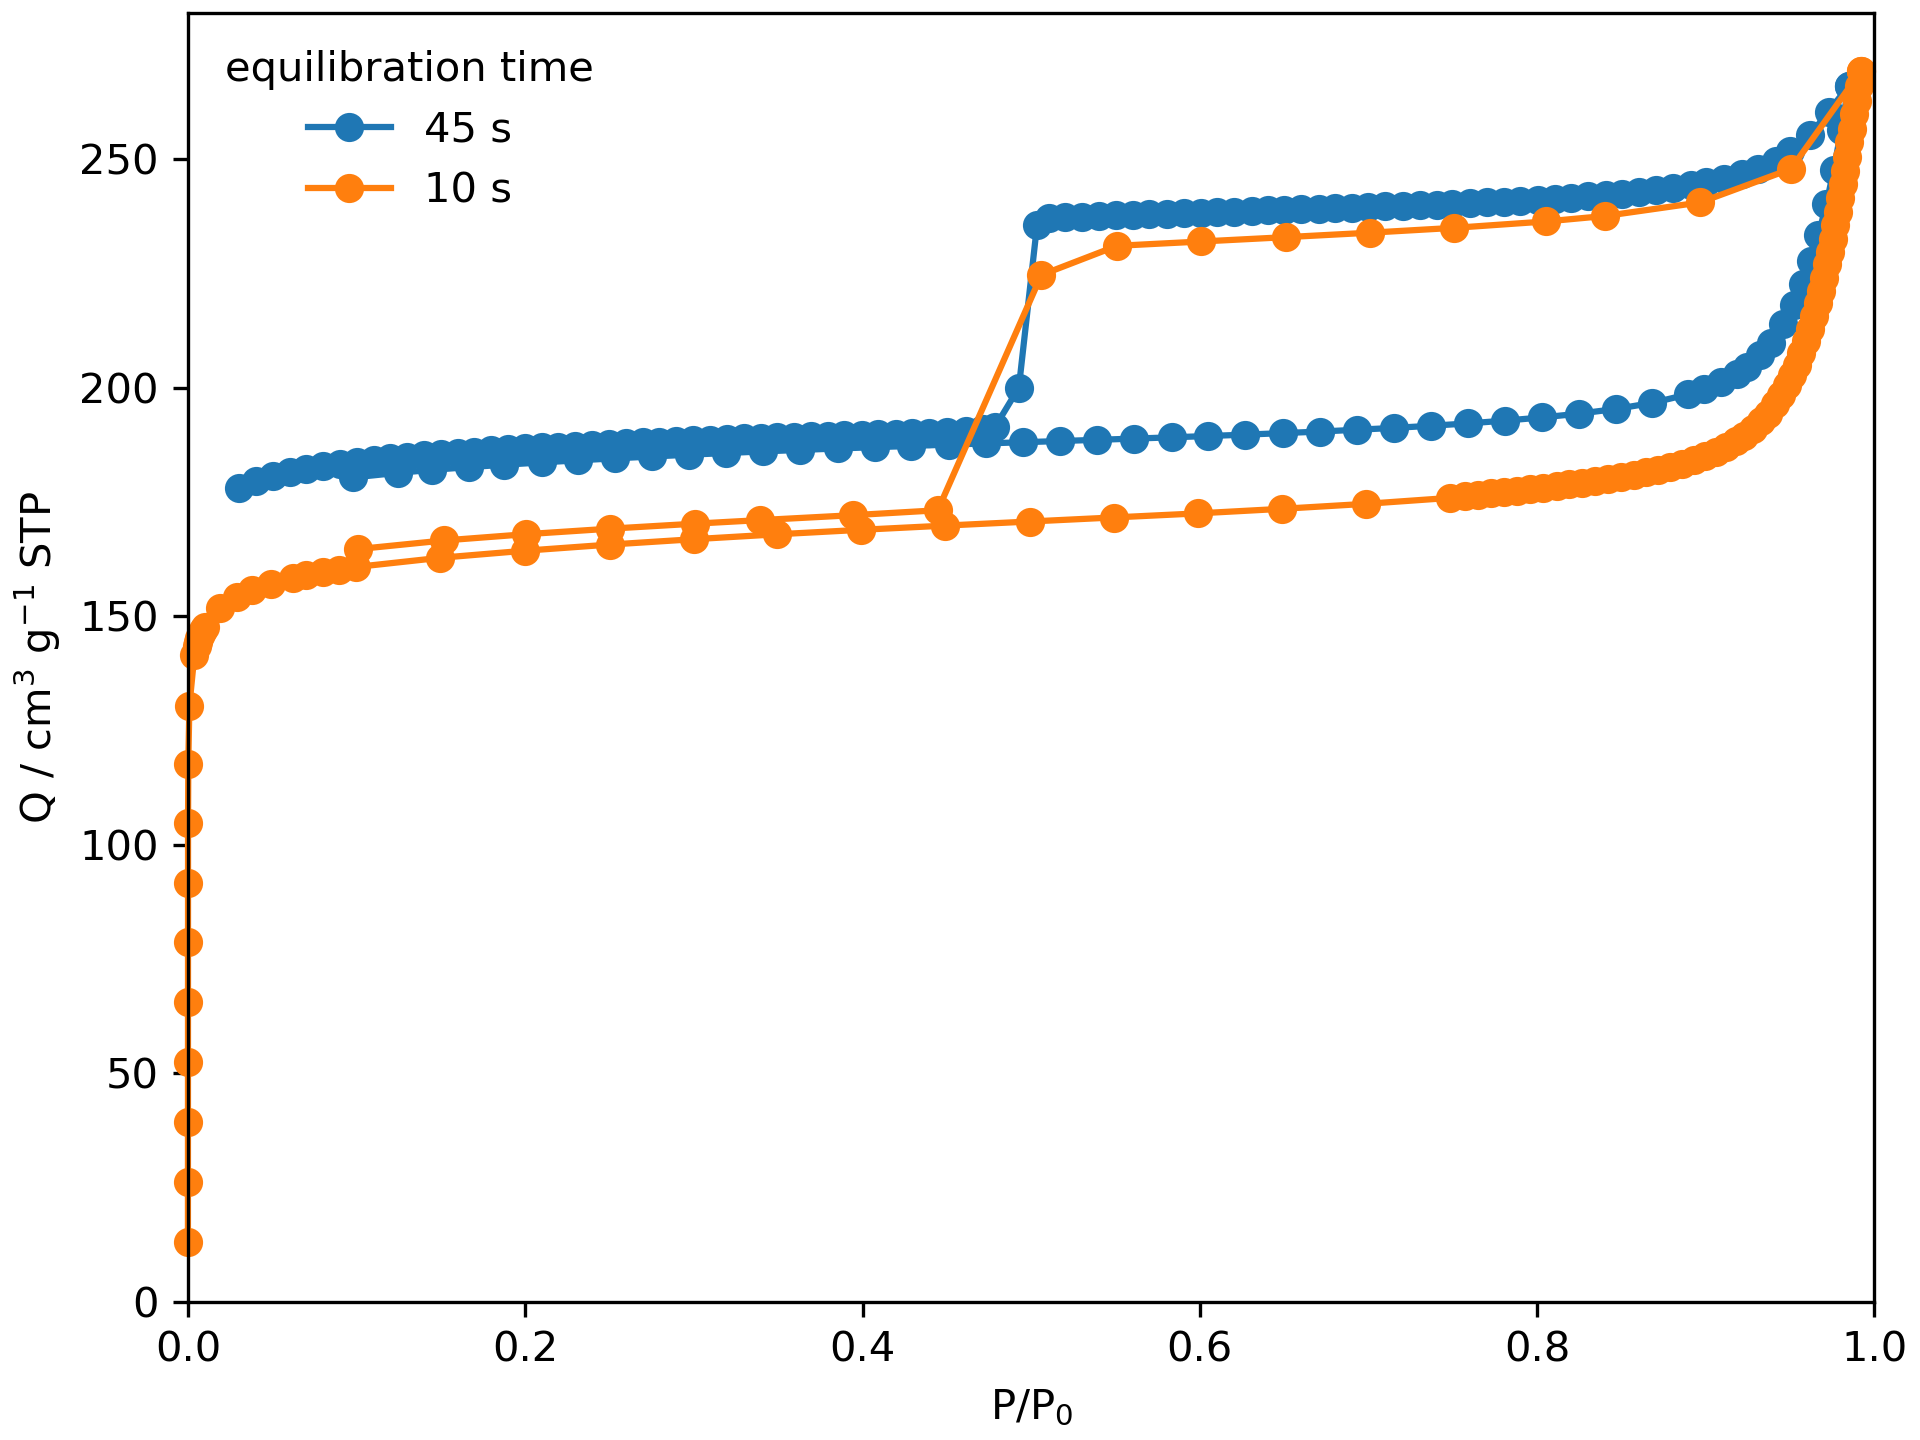
\includegraphics[width=\columnwidth, keepaspectratio]{4-impregnation/figs/hyst.png}
    \caption{Demonstration of the permanence of the hysteresis loop for \ce{N2} isotherms on \acrshort{nc} samples (NC0.9-800 in this case) even when isotherm is given longer to equilibrate during the desorption branch. Small discrepancies in the adsorption branch are likely due to errors in measurement of sample mass.}
    \label{fig:hyst}
\end{figure}

\begin{figure}[hptb]
    \centering
    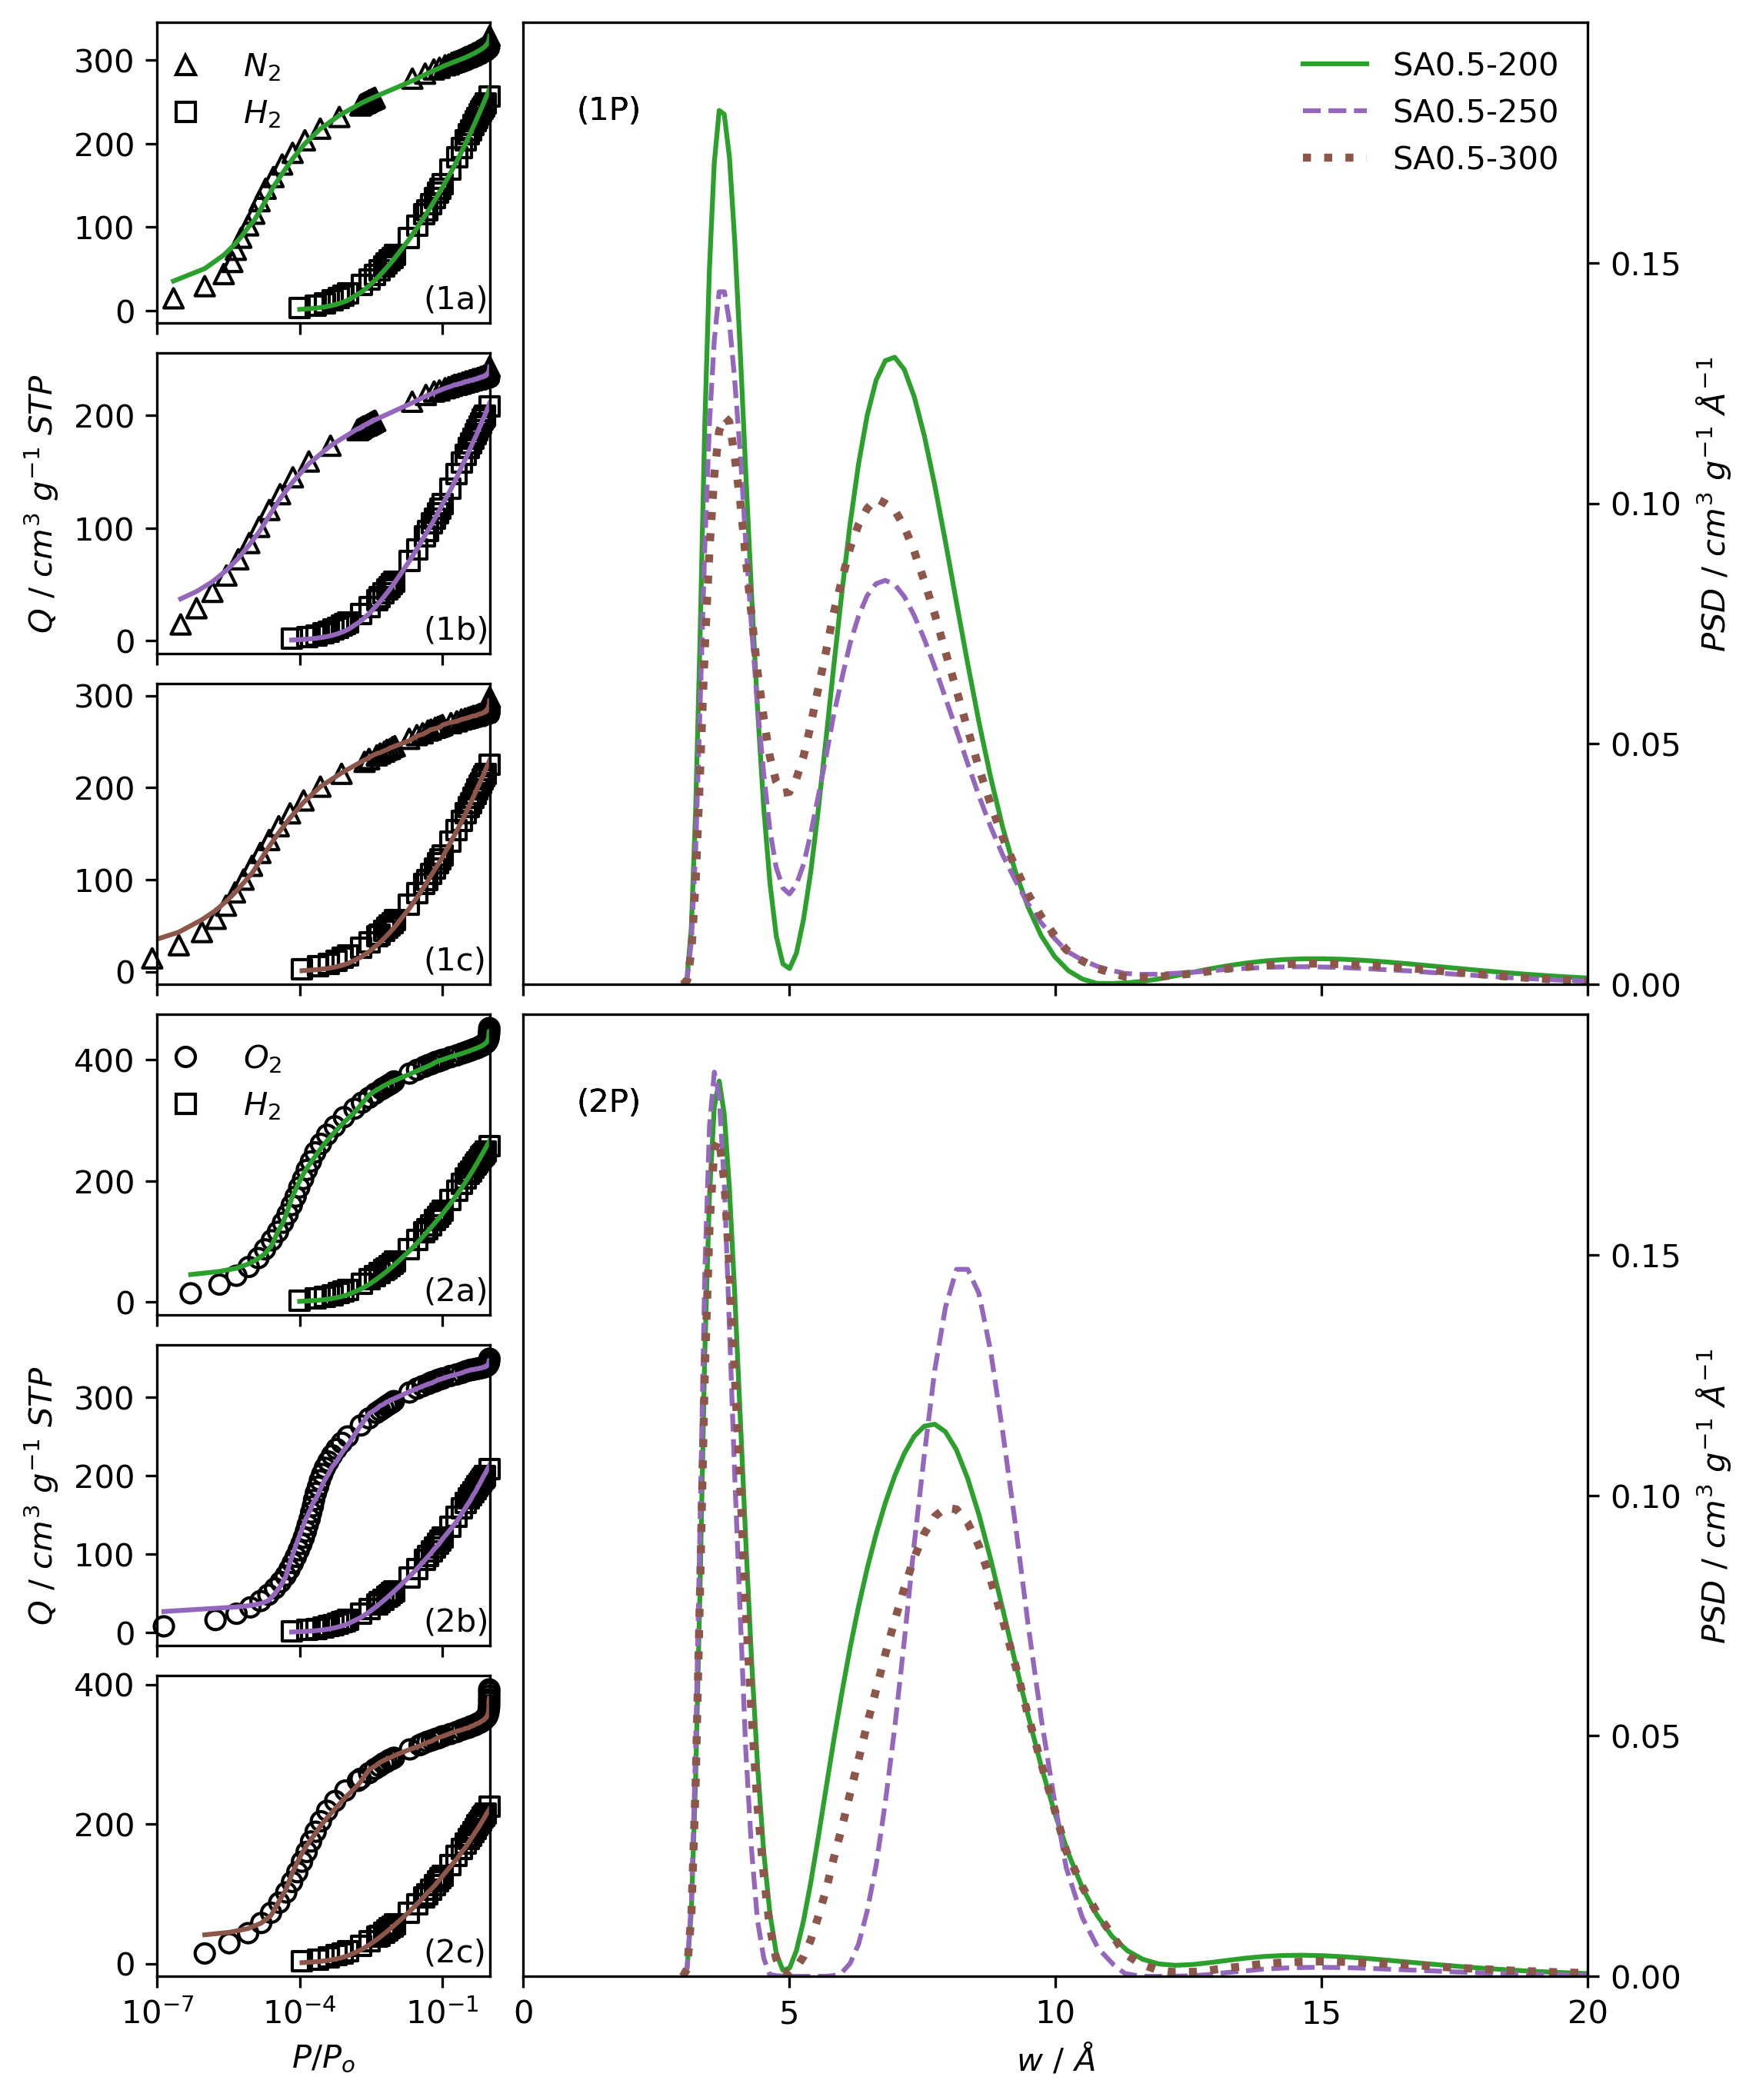
\includegraphics[width=\columnwidth, keepaspectratio]{5-dual_isotherm/figs/SA050-xxx_isopsd.png}
    \caption{Changes in porosity with \gls{htc} temperature for SA0.5-\textit{TTT} carbons. Compared according to dual fit \ce{N2}/\ce{H2} (1) and \ce{O2}/\ce{H2} (2) porosimetry.}
    \label{fig:SA050-xxx_isopsd}
\end{figure}

\begin{figure}[hptb]
    \centering
    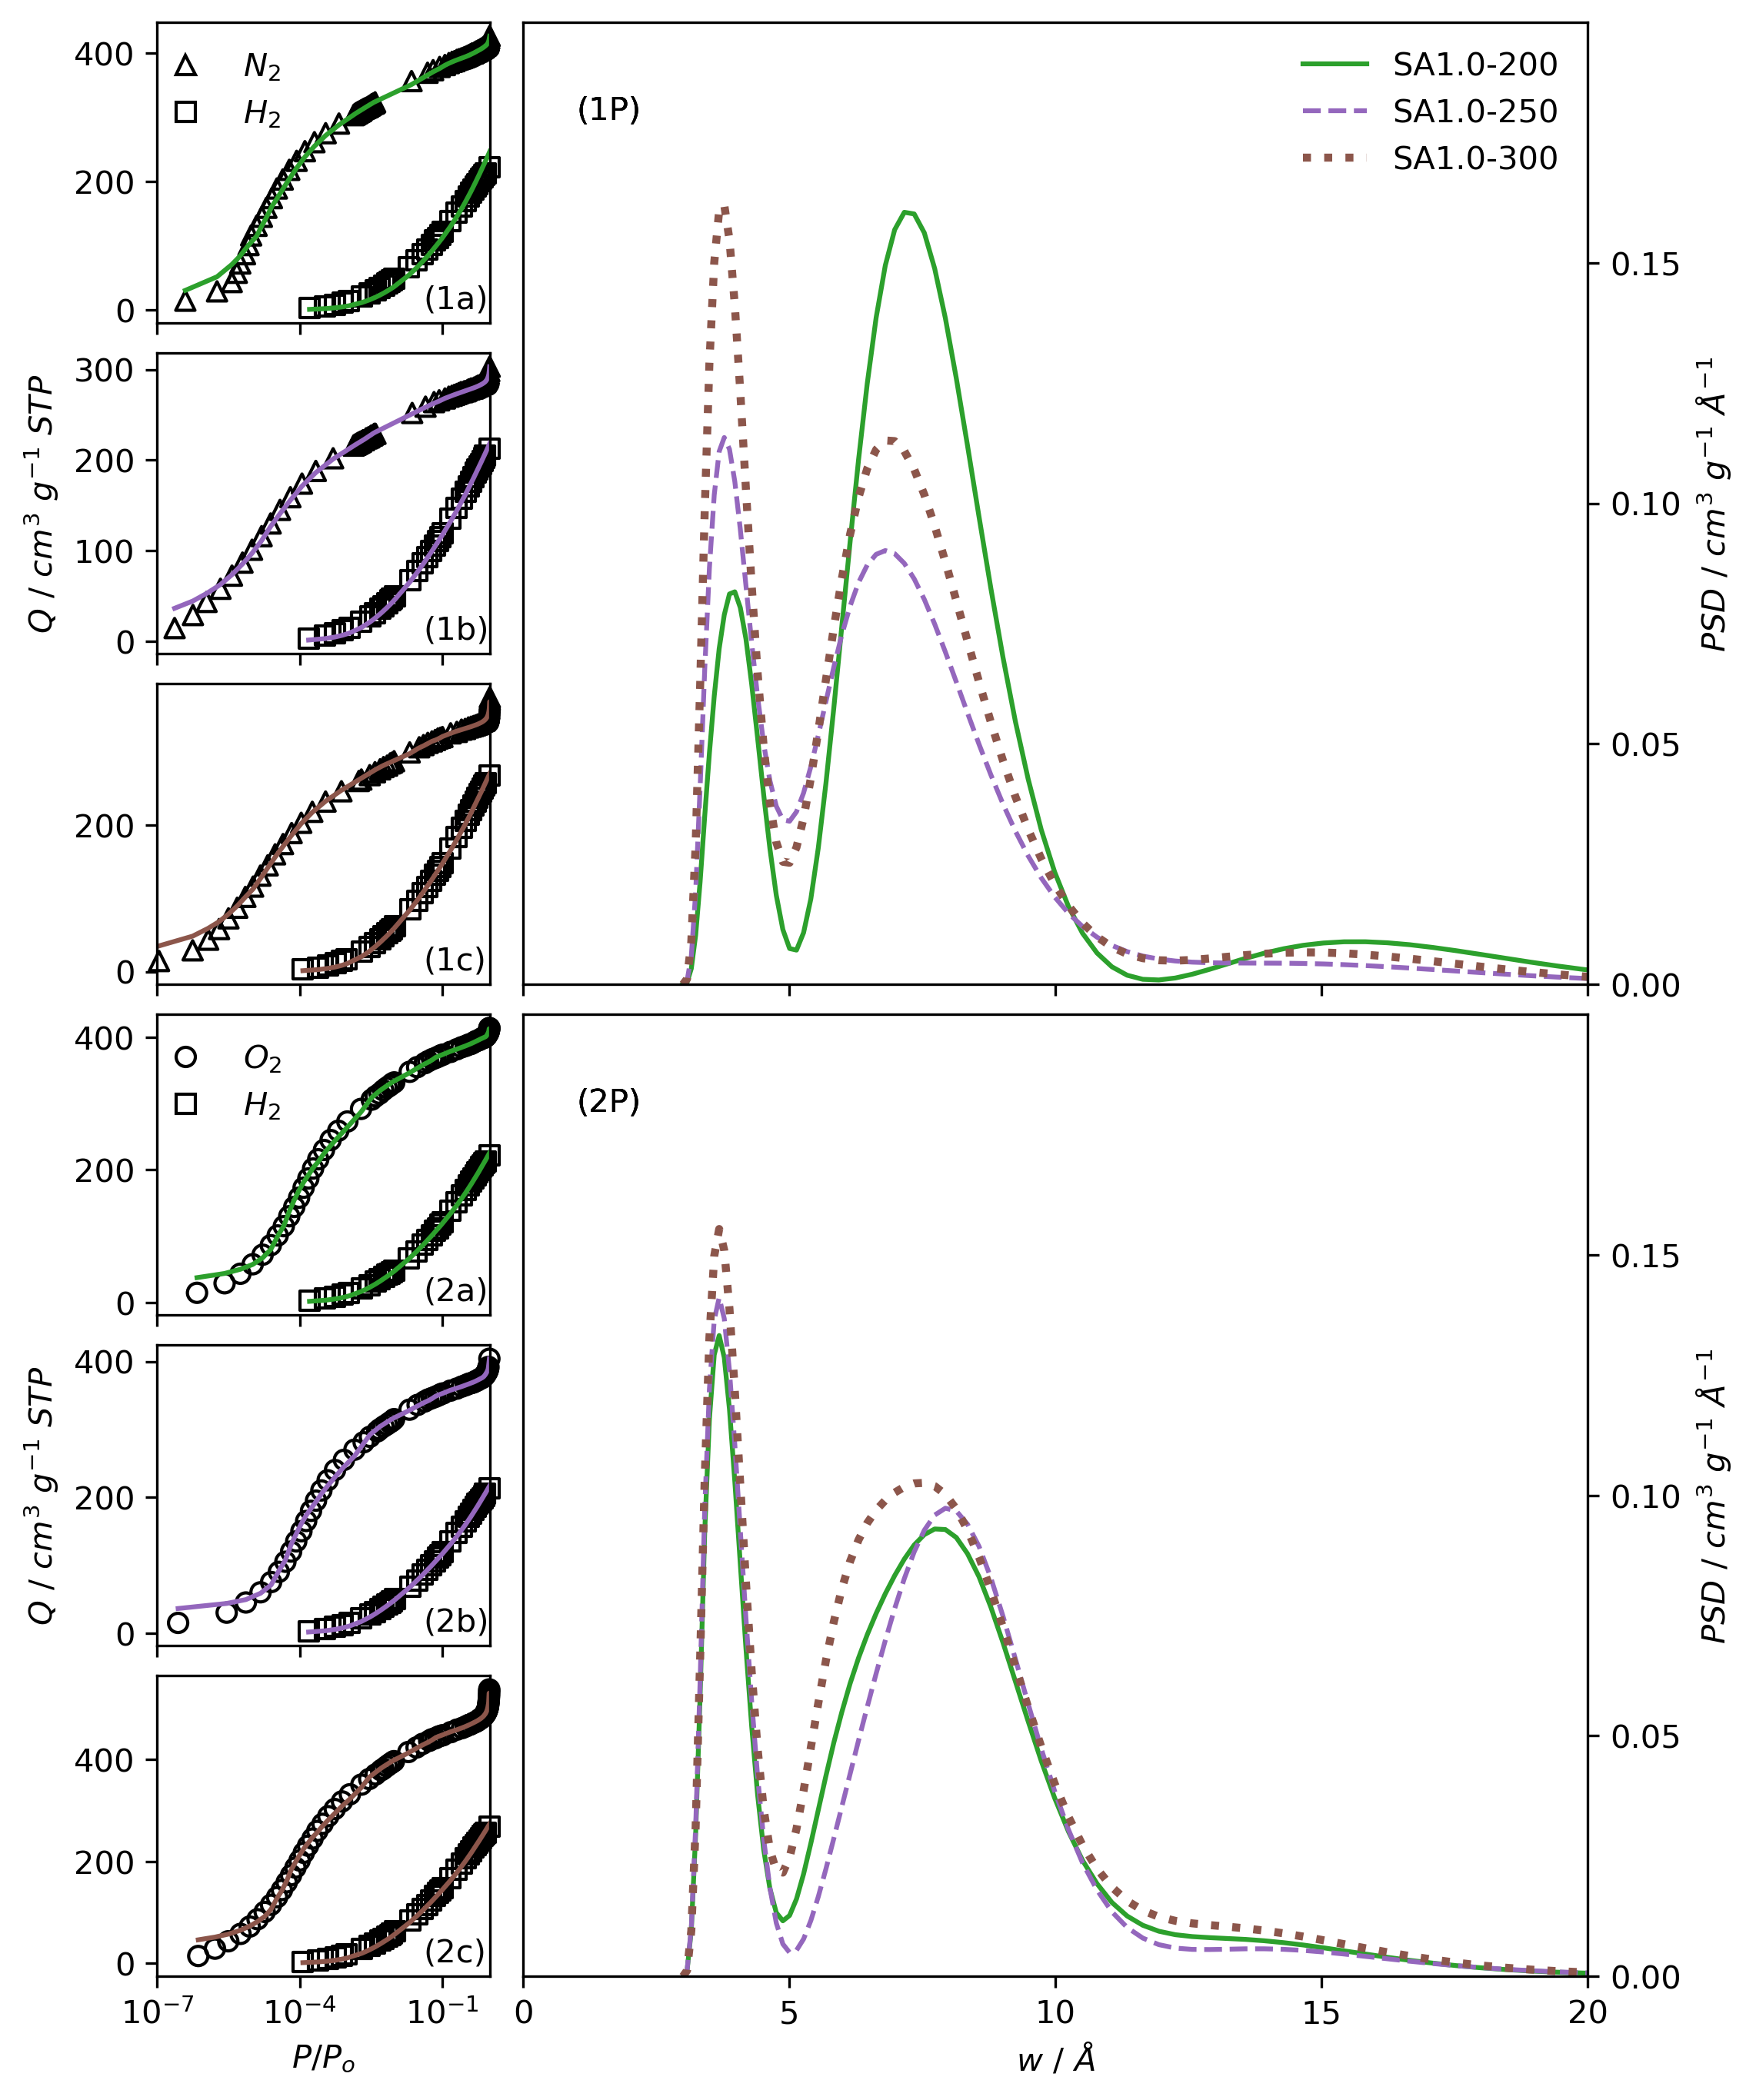
\includegraphics[width=\columnwidth, keepaspectratio]{5-dual_isotherm/figs/SA100-xxx_isopsd.png}
    \caption{Changes in porosity with \gls{htc} temperature for SA1.0-\textit{TTT} carbons. Compared according to dual fit \ce{N2}/\ce{H2} (1) and \ce{O2}/\ce{H2} (2) porosimetry.}
    \label{fig:SA100-xxx_isoposd}
\end{figure}

\chapter{Software}
\newpage

\begin{figure}[h]
\centering
    \begin{verbatim}
        
    Loading DataFrame generated at 15:09 on 22-01-26
    ------------------------------------------------
    
    Project name = 0000_example, Sorptive = co2, T = 298 K
    Models used = ['Langmuir', 'DSLangmuir', 
                    'TSLangmuir', 'GAB', 
                    'Freundlich', 'DR', 'Toth'], 
    Number of isotherms = 4
    Pressure range = 1.0 - 4.0 bar, with increment 1.0
                
    \end{verbatim}
    \captionof{figure}{An example of the report generated after processing experimental uptake isotherms with pyPUC.\\}
    \label{fig:loading_report}
    
    \centering
    \begin{verbatim}
    
    Parameter DataFrame generated at 15:08 on 22-01-26 
    ------------------------------------------------
    
    Project name = 0000_example, Sorptives = n2h2,
    Number of PSDs = 4, calculated for surface area.
    Using pore widths between 4.0 and 7.0 A with a 
    minimum increment of 1.0 A
                
    \end{verbatim}
    \captionof{figure}{An example of the report generated after processing experimental \acrshortpl{psd} with pyPUC.}
    \label{fig:psd_report}
\end{figure}

\end{appendices}


